\documentclass[12pt,a4paper,twoside,openright]{book}

%%%%%%%%%%%%%%%%%%%%%%%%%%%%%%%%%%%%%%%%%%%%%%%%%%%%%%%%%%%%%%%%%%%%
%  Template per Tesi di Laurea                                     %
%                                                                  %
%%%%%%%%%%%%%%%%%%%%%%%%%%%%%%%%%%%%%%%%%%%%%%%%%%%%%%%%%%%%%%%%%%%%

               %%%%%%%%%%%%%%%%%%%%%%%%%%%%%%%%%%%%%%
               %    Scelta dei package da usare     %
               %%%%%%%%%%%%%%%%%%%%%%%%%%%%%%%%%%%%%%


\usepackage[dvips]{graphicx}
\usepackage{graphics}
\usepackage[normalem]{ulem}
\usepackage[utf8]{inputenc}
\usepackage[italian,british]{babel}
\usepackage{float}
\usepackage{graphicx,algorithm,algorithmic}
\usepackage{amsmath,amsfonts,amssymb,amsthm}
\usepackage{epsfig}
\usepackage{deistesi}
\usepackage{fancyhdr}
\usepackage{xspace}
\usepackage[colorlinks=false]{hyperref}
\usepackage[avantgarde]{quotchap}
\renewcommand\chapterheadstartvskip{\vspace*{-5\baselineskip}}
\renewcommand\sectfont{\sffamily\bfseries}
\usepackage{mathptmx}       % selects Times Roman as basic font
\usepackage{helvet}         % selects Helvetica as sans-serif font
\usepackage{courier}        % selects Courier as typewriter font
\usepackage{type1cm}        % activate if the above 3 fonts are
\usepackage{makeidx}         % allows index generation
\usepackage{multicol}        % used for the two-column index
\usepackage[bottom]{footmisc}% places footnotes at page bottom
\usepackage{times}
\usepackage{subfigure}
\usepackage{stmaryrd,mathtools}
\usepackage[noend]{distribalgo}
\usepackage{eurosym}
\usepackage{cleveref}


\newcommand{\bnfs}[0]{\;|\;}
\newcommand{\opar}[0]{\;|\;}
\newcommand{\sq}[0]{\oplus}
\newcommand{\tuple}[2]{#1\langle #2\rangle}
\newcommand{\tupled}[2]{#1[#2]^{\Rightarrow}}
\newcommand{\actrate}[2]{#1^{#2}}
\newcommand{\leave}{{}}
\newcommand{\near}[3]{#1\!\stackrel{#3}{\rightsquigarrow}\!#2 }
\newcommand{\scope}[2]{\llbracket #1 \rrbracket_{#2}}
\newcommand{\law}[1]{[#1]}
\newcommand{\firing}[3]{#1^\rightsquigarrow(#2,#3)}
\newcommand{\shfiring}[1]{#1^\rightsquigarrow}

\newcommand{\defn}[2]{\mathit{def} #1 := #2}
\newcommand{\defnarr}[2]{\mathit{def} #1 & := & #2}
\newcommand{\call}[1]{call\, #1}
\newcommand{\tap}[1]{#1}
\newcommand{\localc}{\texttt{local}}
\newcommand{\neighborhood}{\texttt{neighborhood}}
\newcommand{\globalc}{\texttt{global}}
\newcommand{\lsa}[1]{\langle #1\rangle}
\newcommand{\rem}[1]{+#1}


               %%%%%%%%%%%%%%%%%%%%%%%%%%%%%%%%%%%%%%
               %  Scelta del tipo di font da usare  %
               %%%%%%%%%%%%%%%%%%%%%%%%%%%%%%%%%%%%%%

%\usepackage{times,mathptm}
%\usepackage{palatino,mathpple}
%\usepackage{bookman}
%\usepackage{newcent}

               %%%%%%%%%%%%%%%%%%%%%%%%%%%%%%%%%%%%%%%%
               % Scelta delle dimensioni della pagina %
               %%%%%%%%%%%%%%%%%%%%%%%%%%%%%%%%%%%%%%%%

\setlength{\textwidth}{16.0cm}
\setlength{\textheight}{21cm}
\setlength{\footskip}{3cm}



               %%%%%%%%%%%%%%%%%%%%%%%%%%%%%%%%%%%%%%
               %  Informazioni generali sulla Tesi  %
               %    da usare nell'intestazione      %
               %%%%%%%%%%%%%%%%%%%%%%%%%%%%%%%%%%%%%%

\titolo{Engineering complex computational ecosystems}
\candidato{Danilo Pianini}
\annoaccademico{2015}
\facolta{Ingegneria}
\dipartimento{DEIS - Dipartimento di Elettronica, Informatica e Sistemistica}
\dottorato{PhD Course in Electronics, Computer Science and Telecommunications}
\settoreconcorsuale{09/H1}
\settoredisciplinare{ING-INF/05}
\ciclo{XXVII}
\tutor{Antonio Natali}
\relatore{Mirko Viroli}
% \correlatoreb{Andrea Roli}
% \correlatorec{Mirko Viroli}
\coordinatore{Alessandro Vanelli Coralli}
\dedica{
\emph{\mbox{~~~~~~~~~~~~~~~~~~~~~~~~~~~~~~~~~~~~~~~}Lorem ipsum dolor sit amet. \\
%
\mbox{~~~~~~~~~~~~~~~~~~~~~~~~~~~~~~~~~~~~~~~~~~~~}consectetur adipiscing elit.\\
%
\mbox{~~~~~~~~~~~~~~~~~~~~~~~~~~~~~~~~~~~~~~~~~~~~}Sed fringilla quis mauris id sagittis everything.}\\ \\ \\ \\
\noindent \emph{\textbf{Acknowledgements}}\\ \\
Curabitur commodo dictum risus laoreet tincidunt. Sed dapibus nec ex sit amet consequat. Quisque cursus est sit amet lectus tempor, nec egestas sapien rutrum. Sed dapibus consequat egestas. Quisque blandit, tellus et molestie interdum, augue est molestie lorem, tristique congue metus massa sed eros. Vivamus fermentum erat a faucibus porta. Praesent sit amet risus leo. Integer venenatis lectus sed euismod euismod. Ut pulvinar fermentum sagittis. Aliquam maximus nisl velit, ac varius tellus dignissim in. Fusce nibh dolor, blandit vel nisl non, vehicula tincidunt lorem. Suspendisse fringilla magna ac justo fermentum, nec accumsan odio sollicitudin. Maecenas consectetur, nulla sit amet ultricies pretium, metus sapien posuere turpis, in lobortis tellus turpis ac ipsum. Aliquam sollicitudin augue a aliquam volutpat. Mauris bibendum nunc id est ullamcorper, nec feugiat elit dapibus.\\
%
Duis tincidunt maximus justo, id convallis mauris mattis congue. Maecenas ullamcorper laoreet lacinia. Praesent luctus dictum metus, sed ultrices dui. Fusce fringilla eu est sit amet porta. Aliquam ornare eleifend congue. Aliquam orci urna, accumsan nec metus a, tincidunt pulvinar augue. Nunc eu vulputate lectus. Morbi placerat varius purus at scelerisque. Mauris malesuada ut massa non porta. Quisque ac efficitur odio. Aliquam scelerisque dapibus felis in ullamcorper. Pellentesque ullamcorper massa quis nibh suscipit elementum. Suspendisse tincidunt, sem non porta consectetur, arcu mauris mollis mi, ut commodo libero diam ut risus.
}
\data{March 2015}
\signature{\emph{Danilo Pianini}}

              %%%%%%%%%%%%%%%%%%%%%%%%%%%%%%%%%%%%%%
               % Fine Preambolo                     %
               % Inizio tesi                        %
               %%%%%%%%%%%%%%%%%%%%%%%%%%%%%%%%%%%%%%

\begin{document}

%%%%%%%%%%%%%%%%%%%%%%%%%
% inizio prefazione
%
% pagina del titolo, indice, sommario
%%%%%%%%%%%%%%%%%%%%%%%%%
\frontmatter
\maketitle
\pagestyle{plain}
\tableofcontents

\chapter*{\centering Abstract}
\addcontentsline{toc}{chapter}{Abstract}

This work presents advancements of the latest three years in the engineering techniques for self-organising pervasive ecosystems of devices and services.
%
The inherent complexity of such systems poses new challenges to those who try to dominate the complexity by applying the principles of engineering.

The recent growth in number and distribution of devices with decent computational and communicational abilities, that got suddenly accelerated with the massive diffusion of smartphones and tablets, is envisioning a world with a much higher density of devices in space.
%
This already high device density is probably going to consistently rise if the diffusion of wearable devices gets momentum.
%
Also, communication technologies seem to be focussing on short-range device-to-device (P2P) interactions, with technologies such as \btle{} and Near-Field Communication getting more and more diffused.

Locality and situatedness become key to provide the best possible experience to users, and the classic model of a centralised, enormously powerful server gathering data and processing it is likely to get less and less efficient with device density.
%
Accomplishing complex global tasks without a centralised controller responsible of aggregating data from devices, however, still is a challenging task.
%
In particular, it is hard to understand which device-local programs could properly interact and guarantee a certain global service level.
%
Such local-to-global issue makes the application of engineering principles challenging at least.

In this work, I lay the foundations of my contribution by first analysing the state of the art in coordination systems, namely in those software frameworks devoted to control and promote interactions among independent software entities.
%
I then motivate my work, by describing the main issues of pre-existing tools and practices and identifying the improvements that would benefit the design of such complex software ecosystems.
%
My contribution is described in \Cref{contribution}, and can be divided in three main branches: i) a novel simulation tool for pervasive ecosystems, ii) introduction of novel and improvements over existing self-organisation patterns, iii) the creation of a new language and interpreter based on ``field calculus'' and its integration with the previously mentioned simulator.
%
Finally, I draw conclusions and future works.

\mainmatter

% stile della pagina
\pagestyle{fancy}
\fancyhead[LE,RO]{\bfseries\thepage}

\part{Background and Motivation}
\label{background}
\chapter{Pervasive devices}
\label{pervasive-devices}

It is no mystery that, with the huge progresses of miniaturisation, computational-capable devices are populating the world.
%
The diffusion got momentum with affordable ``personal computers'' that made their way in a one-device-per-family world.
%
Laptops boosted the process, offering user a personal and mobile device.

The pervasive revolution, however took place when the phones became ``smart'', and with the subsequent improvements in the communication technologies.
%
In this chapter, I try to briefly walk the path of success of personal mobile devices, describing also the probable newcomer, namely the wearable devices.
%
I also focus on the current status of the communication protocols, their range and usage, and I try to foresee which world are we going to build if the current trend continues.

\section{Smart, portable devices}

\begin{figure}
	\centering
	
\includegraphics[width=0.99\textwidth]{img/iphone}
	\caption{Apple iPhone is one of the first devices without any physical keyboard, and the first smartphone to gain worldwide success. \emph{Source: Wikimedia.}}
	\label{img:iphone}
\end{figure}

When Apple in 2007 released the first iPhone (\Cref{img:iphone}), a mobile revolution started.
%
Even though other manufacturers proposed products similar to iPhone under the point of view of communication technologies and computational capabilities in the same time frame (e.g. Nokia N810), the Apple's smartphone was the first gaining widespread adoption.
%
It is not really relevant for this work to understand if the branding, the design, the multi-touch finger based interaction UI or the feature set was the key of its commercial success: what really matters is that, starting 2007, every person began to carry with her a personal device featuring both the abilities to communicate and compute.
%
The reason, besides the success of iPhone in the higher segment of the phone market, is mainly to attribute to the widespread diffusion of similar but cheaper and less powerful devices in the lower segments.
%
This kind of devices ultimately pushed the market share of the dominating today's mobile operating system, Google's Android.

This trend towards a higher diffusion got another leap forward three years later, in 2010, when a device with a feature set similar to iPhone, but with no phone abilities  and a bigger screen was released: the iPad.
%
As iPhone gave new vitality and perspectives to the phone arena, iPad revitalised a market that was languishing: the tablets.
%
Tablet devices as they were conceived before iPad launched were nothing more than small laptops with a screen that could be rotated or detached from the keyboard, and a touch-screen normally used with the help of a pen.
%
They changed from devices designed for a professional niche to widespread tools, up to the point that Gartner forecasts their shipments to overtake in 2015 those of desktop PC and laptops aggregated \footnote{\url{http://www.gartner.com/newsroom/id/2791017}}.

The new frontier of pervasive is probably the wearable technology. Smartphones were precursors, they substituted mobile phones introducing new features and they have potential to substitute our wallets (see, for instance, payments through NFC technology) and keys, becoming the only object we need to carry with us in our pockets.
%
Still there are other accessories which are hard to replace, above all watches and glasses.
%
Yes, smartphone can easily show the current time accurately (and, to be honest, also feature phones had this feature well before 2007), but they require the user to pick them from the pocket, turn them on, and sometimes, depending on privacy settings, also unlock them.
%
The whole operation, takes a much longer time and higher effort with respect to just rotating a wrist.
%
This might be the reason why, despite the explosive expansion of smartphones, the wristwatches market did not declined, as an analysis from MarketWatch points out \footnote{\url{http://www.marketwatch.com/story/the-watchs-time-isnt-up-2013-07-01}}.

\begin{figure}
	\centering
	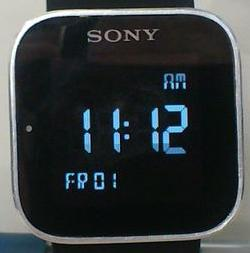
\includegraphics[height=5cm]{img/sony-sw}
	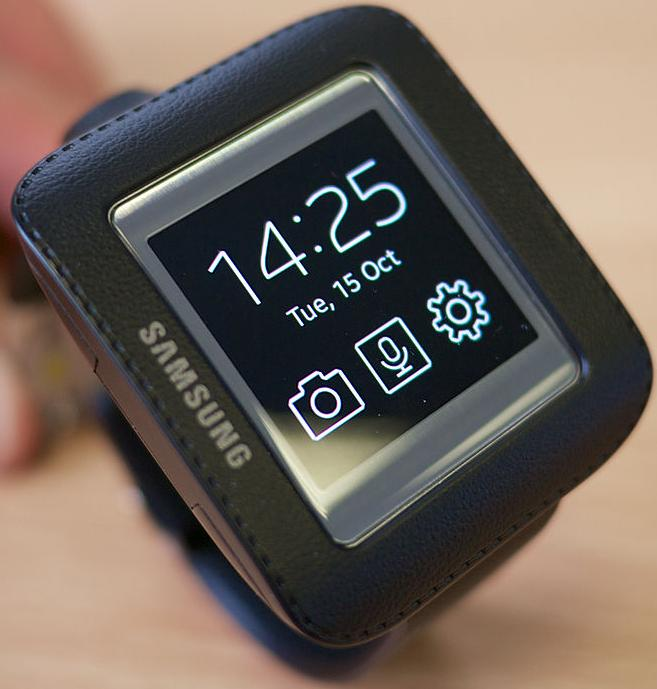
\includegraphics[height=5cm]{img/samsung-gg}
	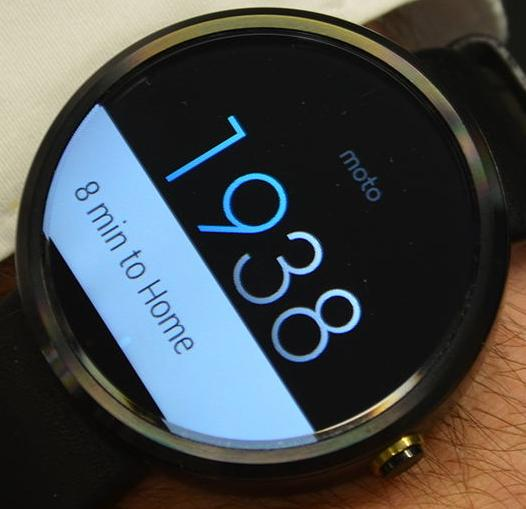
\includegraphics[height=5cm]{img/moto360}
	\caption{Smart watches. From left to right: Sony Smartwatch \emph{(Source: Alex S.H. Lin)}, Samsung Galaxy Gear \emph{(Source: Karlis Dambrans)}, Motorola Moto 360.}
	\label{img:watches}
\end{figure}

There is room for manufacturers to create new portable devices.
%
Sony, starting 2012, has produced a series of smartwatches, such as those in \Cref{img:watches} that pair with a smartphone and provide quick access to some of its functionalities.
%
The success of such solution is not huge, but despite that many other companies are interested in this market: Samsung, Motorola and Apple presented devices meant to replace the classic wristwatch, a clear sign that this market is in expansion.
%
At the time of writing, the main issues that slow the widespread adoption of such solutions are battery duration and dependence on a smartphone.

\begin{figure}
	\centering
	
\includegraphics[width=0.99\textwidth]{img/gglass}
	\caption{Google Glass. In this image, it is possible to see both the camera (on the left hand side) and the semi-transparent head-mounted display. Are those devices going to be part of our everyday life? \emph{Source: Wikimedia.}}
	\label{img:gglass}
\end{figure}

Another notable attempt to make a common accessory smarter is Google Glass project, depicted in \Cref{img:gglass}.
%
Their goal is to enhance the experience of wearing glasses by attaching a device with a camera, an optical head-mounted display, and the abilities to locate itself and communicate with other devices.
%
Google Glass, at the time of writing, are way to expensive (with the kit sold at \$1500) for being able to penetrate the general public, but they are an interesting anticipation of possible future devices.

On the same line of such wearable devices, a discrete success is being achieved by the so called ``fit bands''.
%
They are bracelets equipped with low energy sensors, mainly accelerometers and gyroscopes, which are used to keep track of user's activity.
%
Depending on the model, they can be used to monitor some user's health parameters, such as the number of steps walked per day or heartbeats.
%
They normally work along with another device, a smartphone or a tablet.
%
Such devices, due to their precise market niche and reasonably low price (the Chinese manufacturer Xiaomi recently introduced a low-end wristband at around \$15) are having a notable success.

The wearable devices segment also includes less common devices such as ``smart shoes'' and materials that can be used to make clothing, such as e-textiles.
%
It is a market in expansion, greatly beneficing from recent increases in performance per watt efficiency.
%
If the trend continues, it is likely that we will more and more powerful wearable devices on sale at cheaper and cheaper prices, and a consequent widespread diffusion.
%
The same sort may occur to other parts of our life: kitchen gear, indoor lights and many other objects are getting more and more ``smart'' around us.
%
We may, literally, end up with a world where every single object embeds computational and communicational abilities.

A problem arise: how can software engineers deal with such a complexity?

\section{Communication technologies}

Besides miniaturisation, and as a consequence the increase of computational density in space, another factor played a fundamental role in the world of pervasive computing: the ability to communicate, and in particular the ability to rely on wireless communication, which is of paramount importance when considering mobility.

In later years, many communication means arose.
%
They largely differ in terms of range, protocols, and availability.
%
In this section, I try to resume the most diffused technologies available on today's devices, but the reader is warned: keep in mind that such technologies are evolving very quickly, and the scenario is incredibly fluid.

\subsection{International Mobile Telecommunications}
\label{International Mobile Telecommunications}

This first mean of communication is designed to allow mobile devices to access the Internet from anywhere in the world, relying on the existing mobile phone infrastructure.
%
Such technologies are meant to be used with the standard IP protocols, and they are normally used to get access to public services, in particular to the world wide web.
%
They are not designed for a local peer-to-peer (P2P) communication, and as a consequence they provide no mean to exploit locality.
%
The diffusion of such communication protocols is widespread, in particular among smartphones.
%
Due to the fact that they rely on the mobile phone network, they require a contract with a mobile telecommunications provider, and as such they are much less diffused in tablets and other portable devices.

\begin{figure}
	\centering
	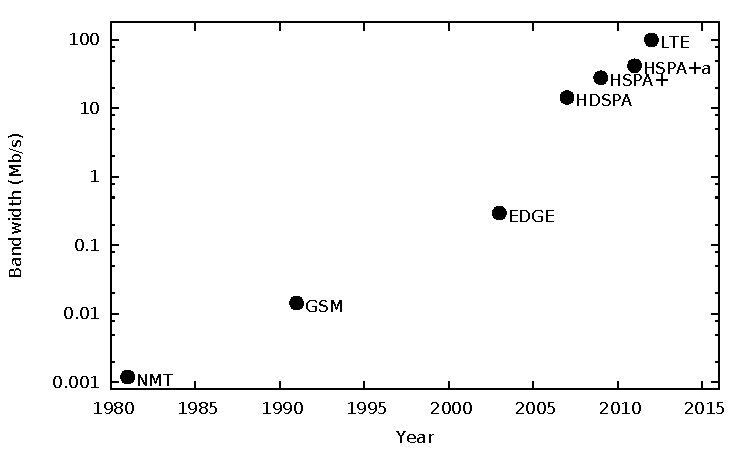
\includegraphics[width=0.99\textwidth]{img/charts/mobile-data-performance}
	\caption{
		Maximum download bandwidth available for mobile devices with time.
		%
		Each point is labelled with the specific communication technology name.
		%
		For the most recent multiple-input-multiple-output (MIMO) technologies, such as LTE, a conservative single input channel was used.
	}
	\label{img:mobile-bandwidth}
\end{figure}

The possibility of accessing the Internet from everywhere is probably one of the key bricks that allowed for the huge success of smartphones in today's world.
%
As \Cref{img:mobile-bandwidth} shows, the bandwidth available grew exponentially with time, to the point that in some countries (e.g. in Italy, at the time of writing) the best available mobile connections offer a higher performance than the best available home connection
%
\footnote{At the time of writing, Telecom Italia Mobile offers mobile connections on LTE with a download bandwidth up to 225Mb/s.
%
Fastweb, the company offering the faster solutions for fiber-to-home connections, goes up to 100Mb/s.}.
%
Such performance unlock the possibility of fully exploiting the possibilities of the world wide web, including cloud services and fruition of multimedia content.

If bandwidth is not currently an issue for international mobile telecommunications, the situation is well different when it comes to device density.
%
Any of us probably experienced network availability issues when participating crowded events, such as concerts or sport events.
%
The current technology, in fact, makes all the network user share the same physical resources: when the device density is too high, there is simply not enough space in the frequency spectrum to grant a decent bandwidth to everyone.
%
Future networks (5G, and presumably those that will follow) are focussing toward this issue among others \cite{5g}.
%
In particular, a so-called ``spectrum crunch'' is expected due to the expected traffic increase (thousand fold over this decade and still growing into the next), that could not be faced simply with the foreseen steady increase of the spectrum allocated for mobile communication, and will require technological advances \cite{spectrum-crunch}.

\subsection{WiFi}

WiFi technology is the most diffused technology for wireless local networking.
%
It is widely diffused, integrated in all smartphones and tablets and also in other devices, such as printers, gaming consoles and TVs.
%
WiFi devices communicate on a distance that ranges from 20 to 100 meters, depending on the condition of the wireless medium and on the power of the communication devices.
%
The communication speed between two linked devices ranges from 56Mb/s to 300Mb/s.

WiFi was designed to provide wireless access to a local area network.
%
In the most classic ``infrastructure mode'', wireless devices get connected to a so called access point, which is responsible to route packets among wireless devices and bridge the wireless local area network to the wired backbone.
%
Multiple access point that share the network name (SSID) may be connected using wired network technologies, and they will appear as a single, bigger access point.
%
It is also possible to drop the wired backbone, but specific access points are required.

Also, some WiFi devices provided ``ad-hoc mode'', allowing multiple devices to directly communicate without an intermediate access point.
%
This working mode was problematic, mainly due to the fact a standard communication protocol for peer-to-peer WiFi communication was missing.
%
This lack was filled with WiFi Direct, which provides a protocol by which one of the devices that want to communicate directly becomes the access point, allowing for direct communication.
%
The most common usage of such a feature are direct file sharing between devices and connection to peripheral devices such as printers or scanners.

\subsection{Bluetooth and Bluetooth LE}

Bluetooth is a technology designed for building energy efficient personal area networks (PANs).
%
Bluetooth devices are assigned a class which identifies the maximum permitted power and, consequently, the maximum operating range.
%
For the most powerful (and power hungry) devices the communication range can go up to 100m.
%
The communication speed ranges from 1Mb/s of the earliest 1.0 version to the 24 Mb/s of version 3.0 and later.

The most interesting features of Bluetooth are not the bandwidth nor the range (WiFi performs better on both), but rather the simple association process and the low power consumption.
%
Thanks to those features Bluetooth found widespread diffusion as a mean to connect low consumption peripherals, such as headsets.
%
Also, it is diffused in cars, and allows user to use the car's audio system as a speakerphone for making calls or listen to music.

\begin{figure}
	\centering
	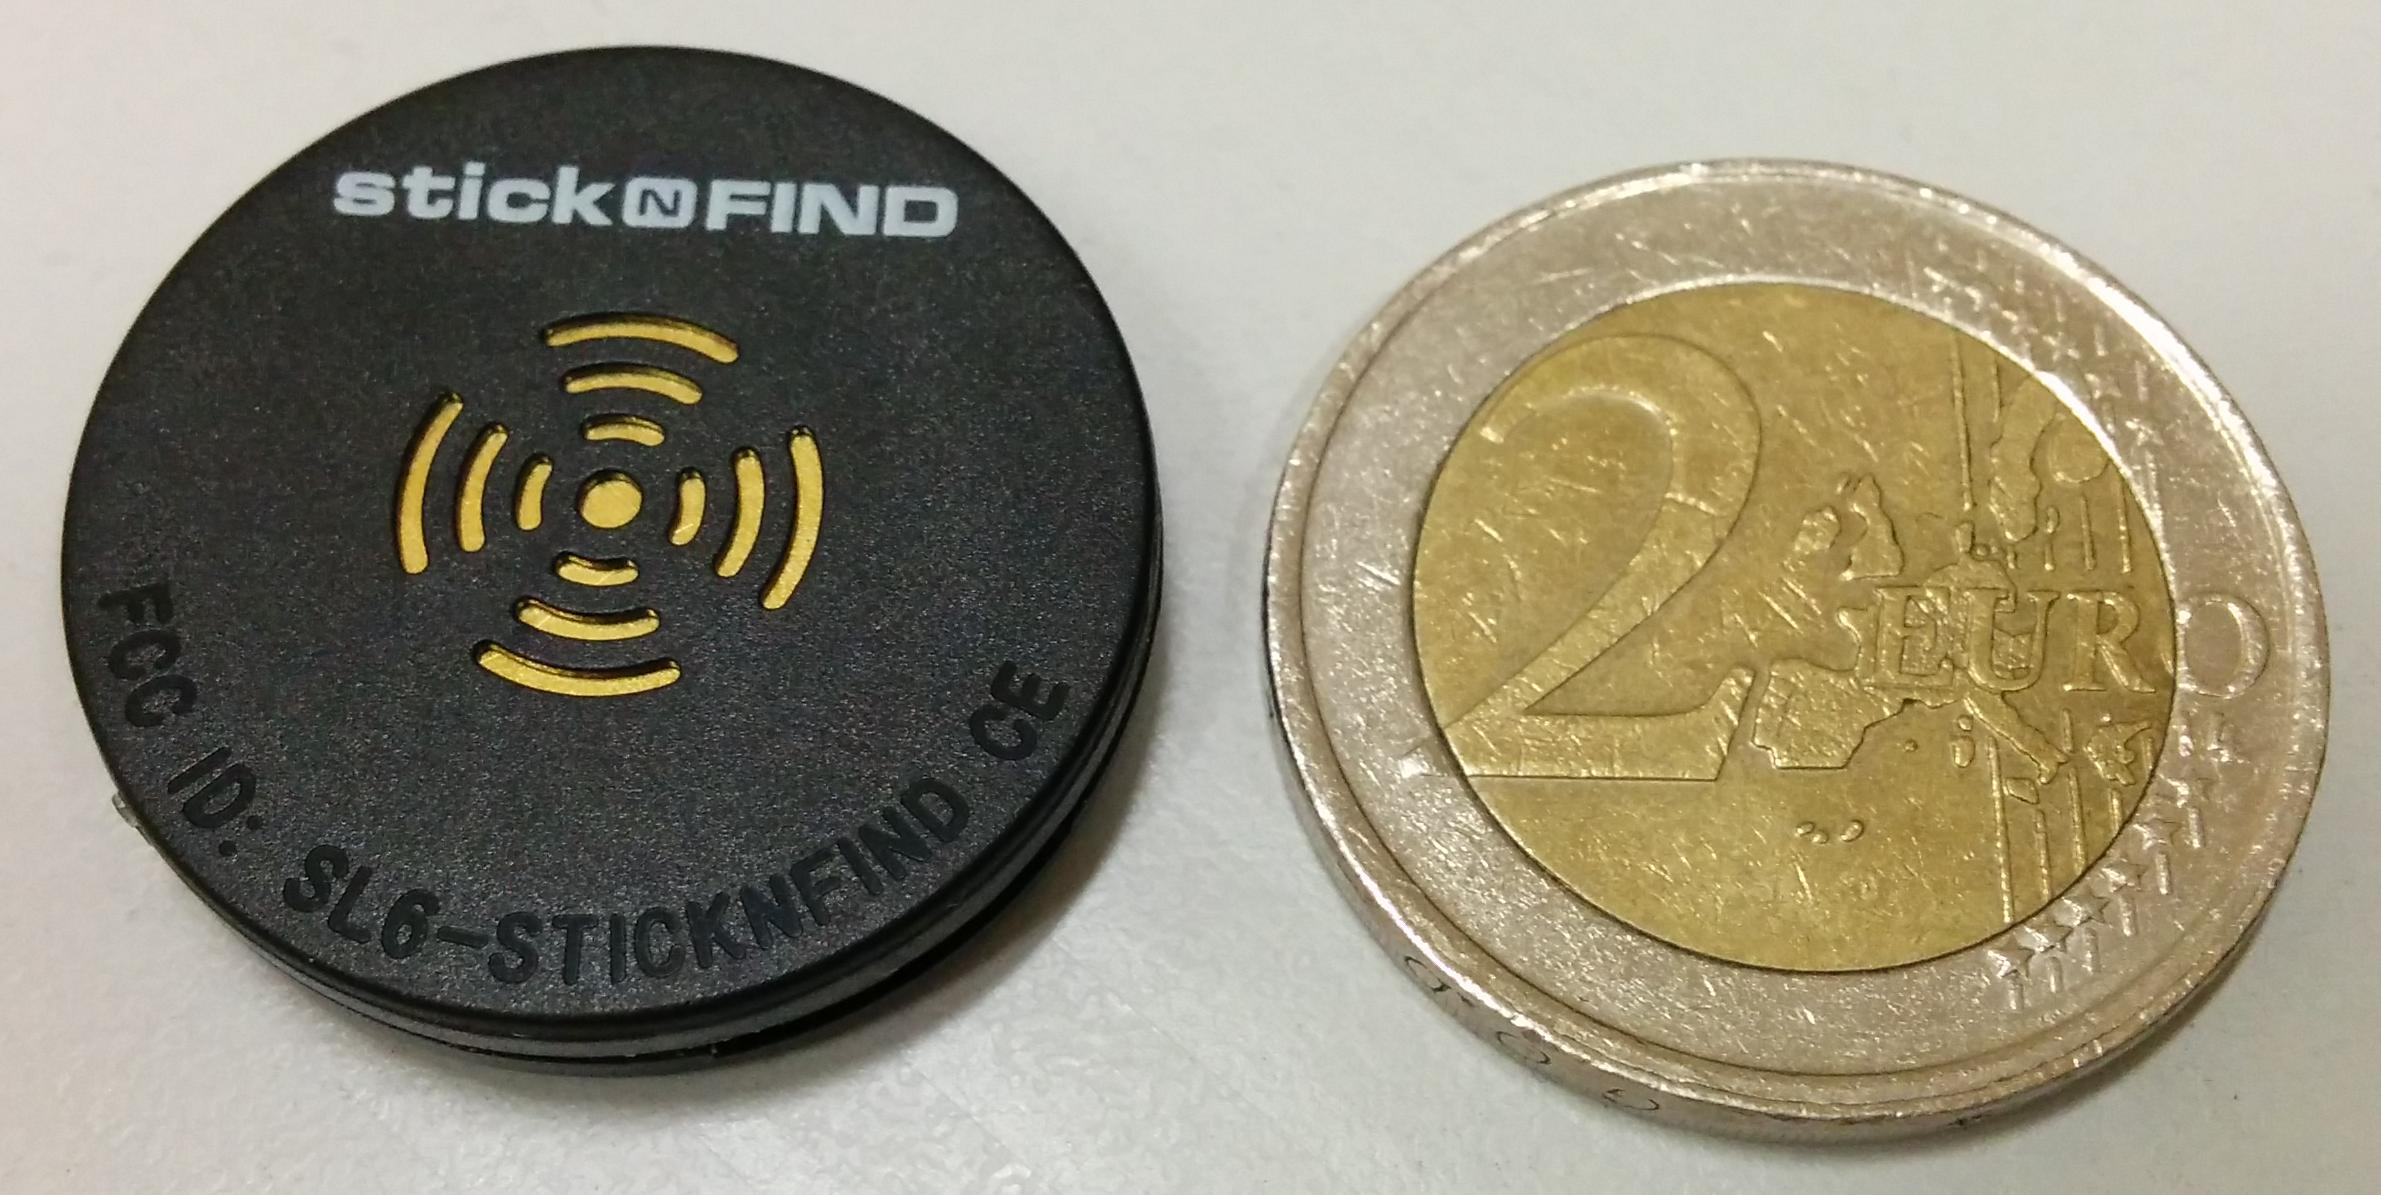
\includegraphics[width=0.99\textwidth]{img/ibeacon}
	\caption{
		A iBeacon, compared to a \EUR{2} coin.
	}
	\label{img:ibeacon}
\end{figure}

A technology which is often associated with Bluetooth but that is actually a separated and not compatible protocol is Bluetooth LE.
%
The reason why such technologies get associated is that, since the radio frequency used is the same (2.4GHz), dual mode devices can share a single radio antenna.
%
LE stands for Low Energy, and it is the main difference between the two protocols: at the expense of some bandwidth, Bluetooth LE consistently reduce the amount of energy required.
%
Bluetooth LE applications are particularly interesting, and range from health care to fitness to alerts to proximity sensing.

Proximity can be estimated using the received signal strength indicator (RSSI), and the very low power consumption of Bluetooth LE allowed for the realisation of electronic leashing systems, namely systems where an electronic device is paired to an object and can be used in order to compute the relative position.
%
The applications are, for instance, finding of misplaced, out-of-sight devices (when the electronic device is paired with a movable object) and indoor localisation (if the electronic device is located on a still standing object).
%
Relying on this technology, Apple created iBeacon, namely very small (coin sized, see \Cref{img:ibeacon}) electronic devices consisting basically of a battery and a Bluetooth LE device.
%
iBeacons can be attached to objects, and they send a universally unique identifier (UUID) to enabled smartphones in range.
%
If the smartphone can associate the UUID with a position, it can deduce its location relative to the iBeacon.
%
The low energy feature plays a fundamental role in this kind of applications: beacons whose battery would last few hours would be of little practical use.
%
With current technologies, a beacon device can be powered by a standard, rather cheap battery for several months, up to a couple of years.
%
This technology is probably the prelude to precise indoor localisation. 

\subsection{NFC}

\begin{figure}
	\centering
	
\includegraphics[width=0.99\textwidth]{img/nfc-tag}
	\caption{
		Two NFC tags, mounted on stickers.
		%
		In order to understand the size, they are placed above a Samsung Galaxy S3, a 4-inches smartphone.
		%
		Moreover, smaller versions of such tags exists, the models pictured here are very common-sized.
	}
	\label{img:nfc-tag}
\end{figure}

Near Field Communication, or NFC, is a technology designed for low energy communication between two devices in proximity (typically few centimetres).
%
It is designed for low energy consumption rather than high bandwidth: its speed (depending on the specification) ranges from 126kb/s to 242kb/s.

One of the most interesting features of NFC is that one of the two devices (the so-called ``tag'') can be completely passive, and still carry a small amount of information within (currently between 96 and 4096 bytes).
%
No battery or energy source is required, the information included can be read by active NFC devices in proximity.
%
Having no need of battery at all, NFC tags can really be tiny, even smaller than iBeacons.
%
\Cref{img:nfc-tag} shows two NFC tags: compared with iBeacons, they can be much lighter and thinner.
%
Brought to the world of humans, it is something like creating a sticker with very small sized text: those who have a powerful enough magnifying glass and are close enough to use it properly can read what it says.

The range of applications of such technology is rather broad.
%
The one which was probably most sponsored is contact-less payment, namely the ability to pay just tapping the phone close to the check-out counter.
%
This is a very interesting possibility, and indeed in 2007 there were enthusiastic forecasts \cite{nfc2007} about its quick diffusion, that did not happen as quick as expected.
%
A number of studies tried to understand the reasons behind this slow adoption, and it appears that reasons are more correlated to marketing and management rather than technological maturity \cite{nfc-diffusion-reasons, nfc-diffusion-europe, nfc-diffusion-asia}.
%
Similarly, if the phone stores identity or access tokens, NFC is a very suitable technology for effectively using such tokens: in this case, its very low range is a nice feature.
%
NFC can also be used as a technology enabler, namely as a mean to securely bootstrap another connection, or join a local network of devices.
%
An example of such use is the Android Beam technology, that relies on NFC in order to establish a Bluetooth connection between two Android devices, transfer a file, then close the Bluetooth connection.
%
Technically, NFC could be used to directly transfer files, but both WiFi and Bluetooth offer much wider bandwidths and range, and as a consequence are preferred for such task.
%
Another interesting application field is mobile device automation: it is achieved by attaching
%
Generally speaking, NFC comes in handy when there is need of a communication mean whose range should be very limited.


\section{Towards a P2P world?}

We are living exciting times.
%
In about five years from the introduction of the technology on the market, almost everybody got a personal smart device always with her.
%
Miniaturisation and power efficiency is constantly growing at a stunning rate, allowing data, communication systems and computation to be spread around in our physical world.

In few decades, we will probably witness the diffusion on computation on everyday object.
%
In such a scenario, the device density will be much higher if compared to the current.
%
One of the possible strategies is to connect every single device to the Internet, aggregate its information in a remote server, do the necessary computation, then send back eventual results where they are needed.
%
This is the strategy behind cloud computing, which is achieving great success.
%
In particular, I argue, this strategy is interesting when the information could or should be aggregated with information from other, distant sources, or conserved for historical purposes.
%
This path, however, gets harder and harder to follow when device density increase: besides the obvious increasing on the total information produced, and consequently of the information to transmit and process, there are two other problems: the saturation of the wireless medium, and the locality of information.

Who tried to use its own smartphone in a very crowded environment has probably experienced connection or network issues.
%
The problem, as discussed in \Cref{International Mobile Telecommunications}, is that current technology must share a common medium among all the devices in the same area.
%
Increasing the maximum number of devices per area is one of the goals of the next generation of international mobile telecommunication technologies.
%
One of the proposed approaches is to switch to a very dense array of very small cells by deploying multiple antennas at a very short distance one another, e.g. inside the public illumination poles.
%
Devices nearby the local antenna would connect to it, and the antenna would then connect them to the rest of the network transparently, in a way somehow similar to the current WiFi ``infrastructure mode''.
%
Clearly, diffusing such antennas can possibly represent a major infrastructural upgrade, and, potentially, cost.

Another observation is that not every device needs direct access to the Internet to be able to accomplish its task, and this is increasingly true with increased density.
%
Thinking about today's devices, let's consider the current smartwatches and fitbands: the former relies on a smartphone or tablet in order to provide Internet-based services, and the latter uses no Internet connection at all, but just sends data to the smartphone to be processed.
%
Along the line of favouring locality, there is a second advantage which relates to privacy issues: there is no reason to send personal information away, if the system does not need data from distant points nor requires more computational power of the amount available locally.
%
Privacy issues gain great attention recently, especially after the leaks of classified information started in 2010 on Wikileaks and continued with the more recent leaks by Edward Snowden.
%
The content of such documents raised greater attention to privacy issues from general public.

A possible path which would help in both those directions (reduce wireless medium usage and keep data as local as possible) is the usage of local, possibly peer-to-peer interactions.
%
This way of organising communication is already exploited by existing applications.

One notable example is Firechat \footnote{\url{https://opengarden.com/firechat}}, which got particularly spotlighted during the ``Umbrella revolution'', namely the sequence of protests that took place in Hong Kong in 2014.
%
Similarly to what was done during Arab springs in 2011 \cite{arab-spring}, protesters relied on Internet services to organise and coordinate themselves.
%
The Chinese government policy on internet is not exactly a bright example of openness and neutrality \cite{china-censorship}, and services such as Facebook adn Twitter, widely exploited during Arab springs, were already effectively blocked in the land.
%
In short time, other social network were closed (such as Instagram), in order to cut protesters' communication means.
%
At that point, protesters had to find a communication system free of centralisation in order to prevent targeted Internet filters, and Firechat was the answer.
%
Firechat is a messaging application for mobile phones that, when the smartphone has access to the remote Firechat cloud, works as other more famous alternatives, such as WhatsApp\footnote{\url{http://www.whatsapp.com/}} and Telegram\footnote{\url{https://telegram.org/}} do.
%
When no access to Firechat servers is available, then the software tries to reach the destination by spreading the message hop-by-hop, building a de-facto mesh network.

Another interesting experiment is Serval Mesh \cite{serval-mesh}.
%
Serval Mesh accomplishes similar tasks, but it also supports calls and file transfers besides messaging.
%
Its main goal is to provide a networking among users who are in an area where there is no Internet access at all, for instance because of a disaster event.
%
It relies on WiFi to create a ad-hoc peer-to-peer network among devices.
%
Due to this lower level aspect, Serval Mesh requires privileged access to the hardware and some higher skill than Firechat, which is easier to setup but requires the availability of a Internet connection.
%
In \cite{mesh-network-telephony}, Serval Mesh is used to build an alternative, purely peer-to-peer telephony network.

Despite the existence of such mesh-oriented applications, however, a general approach for easily design and program such systems is still missing.
%
A consistent part of this work is devoted towards the research of general, well engineered approaches to build such systems.

\chapter{Infrastructures for pervasive computing}
\label{coordination-infrastructures}

In \Cref{pervasive-devices} we took a look to the world of pervasive devices, also describing their communication means and hypothesising the near future development.
%
In this chapter, we focus on the software, and in particular on the challenges of engineering the development of software that will run on an ensemble of pervasive devices.
%
We first discuss the issue of coordination: how do we make all those possibly devices collaborate together in order to achieve a global goal, without a centralised decision-maker?
%
Which software platform may we devise to ease this operation?
%
We will see that similar problems have already been successfully solved in nature: the mechanisms underlying such natural behaviours, can, if properly mimicked, help to realise solutions in software systems.
%
We will then run through the existing literature on the issue, analysing the existing platforms supporting pervasive computing, and the tools that can be used to test and debug applications prior to deployment.
%
Finally, we will discuss the shortcomings of the existing technology, and pave the way for the contribution of this PhD thesis.

\section{Software ecosystems}

When we name pervasive systems, we inherently talk about a multitude of interacting software systems.
%



why do we want a middleware
\section{Nature inspiration}
see what exists, mimic
\section{Coordination platforms and languages}
what is there already
\subsection{Linda}
and swarmlinda
\subsection{Lime}
\cite{murphy2006lime}
\subsection{TOTA}
\cite{mamei2009acm}
\subsection{Plastic}
\cite{plastic}
\subsection{MARS}
\subsection{SELFMAN}
\cite{selfman}
\subsection{TuCSoN}
\cite{tucson-aamas99}
and the semantic extension
\subsection{Biochemical tuple spaces}
and MoK?
\subsection{CArtAgO}
\cite{RPV-JAAMAS2011}
\subsection{SAPERE}
general idea of sapere, grounds on previous works.
\subsection{Proto and Field Calculus}
\subsubsection{Alignment}
\section{Spatial patterns}
what is a pattern
patterns before sapere (gossip, gradient)
problems with gradient

\section{Engineering and tools}
\label{engineering-and-tools}
% JOS %
Development methodology for complex pervasive systems always include \emph{simulation} as a key step \cite{MCOV-SCP2011,BabulakIJOE2008,BandiniJASSS2009,josMacalN10} to realise what-if analysis prior to actual development, to both assess the general validity of the designed mechanisms and to fine tune system parameters.
%
There are many kinds of simulation tools available: they either provide programming/specification languages devoted to ease construction of the simulation process, especially targeting computing and social simulation (e.g. as in the case of multi-agent based simulation \cite{BandiniJASSS2009,SchumacherCEEMAS2007,vizzari-massimulationbook09,repast,sklar2007al}), or they stick to quite foundational computing languages to better tackle performance, mostly used in biology-oriented applications \cite{Priami1995,murata1989,UhrmacherWSC2005,EwaldJOS2007}.
%
None of the existing tools, however, aims at bridging the gap between these approaches, trying to extend the basic computing model of chemical reactions -- still retaining its high performance -- toward ease applicability to complex situated computational systems.


methodological issues, deployment and testing issues, need of simulation
\subsection{General purpose frameworks}
MASON \cite{luke2005simulation}, Repast \cite{repast}, NetLogo \cite{sklar2007al} and Swarm
\subsection{Specific simulators}
network simulators (the one, ns2)
biological simulators (ask Sara)

Specific per-use simulators, gener

\chapter{Shortcomings of coordination infrastructures}
\section{Engineering emergence}
\section{Local to global}
\chapter{Shortcomings of existing tools}
\section{Specific tools: expressiveness}
\section{General purpose tools: performance}

\part{Contribution}
\label{contribution}
\chapter{An integrated toolchain for pervasive ecosystems}

We discussed in \Cref{engineering-and-tools} the importance of simulation in the engineering process of designing pervasive ecosystems.
%
In this chapter, we will discuss one of my contribution to this research branch, namely the development of an integrated tool named \alchemist{}, which has been inspired by chemical oriented simulators.
%
We first talk about chemical inspiration, and how existing chemical-oriented stochastic simulation algorithms (SSAs) can be extended towards higher flexibility, up to the point that they become suitable to simulate potentially complex environments, still retaining their high performance.
%
To do so, our first effort will be to take an efficient SSA implementation and convert it to a general-purpose discrete event simulator (DES).
%
We then devise a meta-meta-model, complex and flexible enough to support the definition of middleware-specific meta-models.
%
Finally, some meta-models are presented.
%TODO: expand
%

\section{Chemical-inspired engine}
\label{chemical-engine}
In the following, we present a discrete event simulation engine derived from the popular and successful Gillespie's stochastic simulation algorithm \cite{gillespie1977}, and in particular from its notable and more efficient extensions developed by Gibson-Bruck \cite{gibson2000} and by Slepoy \cite{slepoy2008}.   
%
Gillespie's SSA is a discrete and stochastic method that intrinsically owns the event-driven properties \cite{spatialeventgillespie}: introduced to model chemical systems, nowadays it represents the basis of many simulation platforms, in particular those developed for the investigation of biochemical systems \cite{Priami:2001,Kierzek01032002,CiocchettaH09,versari08,montagna-cs2bio10,btssoc-jos7,Hoops15122006}. 
%
With significative extensions, it was recently used to model artificial systems grounding on computational models inspired to chemical natural systems and ecology \cite{Montagna-MONET2012}.
%
Moreover, its optimised extensions \cite{gibson2000,slepoy2008} are very efficient, thus allowing really fast simulation runs.

%-------------------------------------------------------------------------------
\subsection{Gillespie's SSA as an event-driven algorithm}
%-------------------------------------------------------------------------------
First of all, we summarise the idea that the Gillespie's SSA is grounded on:
%
a chemical system is modelled as a single space filled with molecules that may interact through a number of reactions describing how they combine. 
%
The instantaneous speed of a reaction is called propensity and depends on the kinetic  rate of the reaction and on the number of molecules of all the reagents involved. 
%
For a reaction $i$ of the form:
$$ R_0 + R_1 \xrightarrow{r} P_0 + P_1 + \ldots + P_n$$
the propensity $a_i$ is defined as:
$$ a_i = r\cdot [R_0] \cdot [R_1] $$
where $[M]$ is the number of molecules of species $M$.
%
Given that, the algorithm relies on the idea that the system can be simulated by effectively executing the reactions one by one and changing the system status accordingly. 
%
Every algorithm follows four main steps:
%
\begin{enumerate}
	\item select the next reaction $\mu$ to be executed;
	\item calculate the time of occurrence of $\mu$ according to an exponential time distribution and make it the current simulation time;
	\item change the environment status in order to reflect this execution;
	\item update the propensities of the reactions.
\end{enumerate}
%
Such algorithm is event-driven in that it executes only one reaction/event at a time: it changes the state of the system and consequently the event list \emph{i.e.}. which other reactions/events can be executed from there.

%-------------------------------------------------------------------------------
\subsection{Gillespie's optimised versions}
%-------------------------------------------------------------------------------
This algorithm has been improved in various works in literature, particularly notable is the work in \cite{gibson2000} and \cite{slepoy2008}.
%
Both works optimise the base algorithm in two phases: the selection of the next reaction to execute and the update of the reaction pool -- pending event list -- once an event has been executed.
%
For the latter, they both rely on the concept of ``dependency graph''.
%
A dependency graph (DG) is a statically created directed graph in which nodes are all the reactions in the simulated system, and arcs connect a reaction \texttt{r} to all those that depend on it, namely, those whose triggering time should be updated as $r$ is executed.
%
For instance, if \texttt{r} changes the concentration of some molecule \texttt{m}, all those reactions that use \texttt{m} are to be properly re-scheduled as soon as \texttt{r} is fired.
%
Even though this optimisation does not affect the execution time in the worst case, it offers great benefits in the average case, since most of the reactions are not interdependent.

The selection of the next reaction to execute is where those improved algorithms differ most.
%
In Slepoy's work, the author divides reactions in groups based on their propensity: if $p_{min}$ is the lowest propensity, the first group contains those reactions whose propensity ranges from $p_{min}$ and $2 p_{min}$, the second those between $2 p_{min}$ and $4 p_{min}$, and so on.
%
Give those groups, an algorithm called ``Composition-Rejection'' (CR) is applied.
%
In the composition phase, a group is randomly selected in logarithmic time; in the rejection phase a reaction is chosen within a group by throwing two random numbers: the first one, between $0$ and the number of reactions in the group, identifies a reaction; the second one, between $0$ and the maximum propensity allowed for the group, is used to decide whether or not to actually execute the selected reaction.
%
In case the reaction is rejected, the rejection procedure is re-applied.
%
Given the way groups are built, there is at least a 0.5 probability that the rejection procedure concludes at each attempt.
%
On average, the CR algorithm requires five random numbers to be thrown.
%
This algorithm requires logarithmic time to select the next reaction with respect to the total number of groups, but the author argues which, since in most biological scenarios this number is constant, then the algorithm runs effectively in constant time.
%
In Gibson-Bruck, the same selection operation is made by computing a putative execution time for each reaction, and then using a binary heap data structure to sort them.
%
This way, the next reaction to execute is always the root node of the tree, and the selection is performed in constant time.
%
However, once the reaction has been executed, all the dependent reactions must be updated and re-sorted in the tree. In the worst case, this takes logarithmic time with respect to the number of reactions.

%-------------------------------------------------------------------------------
\subsection{From SSA to full fledged DES}
%-------------------------------------------------------------------------------

Both the Gisbon-Bruck's and Slepoy's schedulers are granted to correctly simulate a Poisson process.
%
However, in order to build a full-fledged DES engine, we must offer the possibility to schedule also non-Markovian events.
%
Imagine, for instance, that we want to simulate an agent that does an action every fixed time interval (e.g. a man walking).
%
This, clearly, is not a memoryless process.
%
We argue that Gibson-Bruck offers a more suitable base for a general purpose DES: in fact, its next reaction choosing mechanism is orthogonal to the way the putative times are computed.
%
This intrinsic feature allows to neatly separate the generation of times (namely, the time distribution of each event) and the actual scheduling (choice of which event should run next).
%
We chose the Next Reaction Method for \alchemist{}, and, consequently, the main simulation algorithm follows the basic steps listed in \Cref{algo:engine}.

\begin{algorithm}
\begin{distribalgo}[1]
\vspace{5pt}
\STATE{\texttt{cur\_time} $=$ 0}
\STATE{\texttt{cur\_step} $=$ 0}
\FOR{each node \texttt{n} in environment}
  \FOR{each reaction \texttt{nr} in \texttt{n}}
    \STATE{generate a new putative time for \texttt{nr}}
    \STATE{insert \texttt{nr} in DIPQ}
    \STATE{generate dependencies for \texttt{nr}}
  \ENDFOR
\ENDFOR
\WHILE{\texttt{cur\_time} $<$ \texttt{max\_time} \AND \texttt{cur\_step} $<$ \texttt{max\_step}}
  \STATE{\texttt{r} $=$ the next reaction to execute}
    \IF{\texttt{r}'s conditions are verified}
      \STATE{execute all the actions of \texttt{r}}
      \FOR{each reaction \texttt{rd} which depends on \texttt{r}}
	\STATE{update the putative execution time}
      \ENDFOR
    \ENDIF
    \STATE{generate a new putative time for \texttt{r}}
\ENDWHILE
\caption{Simulation flow in \alchemist{}}
\label{algo:engine}
\end{distribalgo}
\end{algorithm}

A second feature that we need in order to shift the paradigm from pure chemistry towards higher expressiveness is the possibility to simulate multiple, separate, interacting and possible mobile entities.
%
This requirement can be partly addressed by the notion of intercommunicating compartments \cite{CiocchettaH09,versari08,montagna-cs2bio10,btssoc-jos7}, in a way that allows to also model systems characterised by a set of connected volumes and not only a unique chemical solution.
%
The hardest challenge in simulating multiple compartments with an efficient SSA is in improving the dependency graph: reactions that could be interdependent but happen on separated compartments should not be marked as interconnected within the dependency graph.
%
Mobility makes everything even harder, since it may lead to the creation and disruption of communication channels between compartments, and consequently to simulation-time changes in the structure of such dependency graph.
%
Summarising, supporting dynamic environments with multiple mobile compartments require the dependency graph to become a dynamic data structure, which cannot be pre-computed at the simulation initialisation and kept static.

\subsubsection{Dynamic Dependency Graph}

There are multiple ways to conceive such dynamic data structure.
%
Ideally, it would be possible to just drop the optimisation or reuse the classic definition, in which case the triggering of a reaction in whichever compartment would cause the recalculation of the status of each potentially dependent event in every compartment.
%
This approach would lead to a massive performance impact, since the dependency computation is the most expensive operation.
%
As evidence, in \cite{slepoy2008} some charts show the difference between Gibson-Bruck and Slepoy et al. algorithms with and without a dependency graph: the result is very strongly in favour of the former.

A possibility for efficiently adapting a dependency graph to a network of compartments could be to define the input and output contexts for each reaction, namely the places where reactions respectively ``read'' their reactants and ``write'' their products.
%
Multiple contexts could be defined, we propose to adopt three levels: \localc{}, \neighborhood{} and \globalc{}.
%
In a purely chemical simulation, all the reactions have a \localc{} input context and may have either \neighborhood{} or \localc{} output context, depending on whether or not they send molecules towards other compartments.

Let $dep: R^2 \longrightarrow boolean$ be the function that is used to build the static dependency graph in every SSA: given two reactions \texttt{r1} and \texttt{r2}, $dep(\texttt{r1}, \texttt{r2})$ returns \texttt{true} if the propensity of \texttt{r2} may be influenced by the execution of \texttt{r1}.
%
In a multi-compartment scenario, \texttt{r1} influences \texttt{r2} (there is an oriented edge in the dependency graph connecting \texttt{r1} to \texttt{r2}) iff $dep(\texttt{r1},\texttt{r2})$ is \texttt{true} and:
\begin{itemize}
 \item \texttt{r1} and \texttt{r2} are on the same node OR
 \item \texttt{r1}'s output context is \globalc{} OR
 \item \texttt{r2}'s input context is \globalc{} OR
 \item \texttt{r1}'s output context is \neighborhood{} and \texttt{r2}'s node is in \texttt{r1}'s node neighbourhood OR
 \item \texttt{r2}'s input context is \neighborhood{} and \texttt{r1}'s node is in \texttt{r2}'s node neighbourhood OR
 \item \texttt{r1}'s output context and \texttt{r2}'s input context are both \neighborhood\ and the neighbourhoods of their nodes have at least one common node. 
\end{itemize}
%
The filters listed above greatly compact the number of edges of a dependency graph in most scenarios, with great benefits on the engine performance.
%
On top of this finer-grain locality concept, if the model supports compartment mobility, the dependency graph must support the dynamic addition and removal of reactions.

Adding a new reaction implies to verify its dependencies against every reaction of the system. In case there is a dependency, it must be added to the dependency graph. 
Removing a reaction \texttt{r} requires to delete all dependencies in which \texttt{r} is involved both as influencing and influenced.
Moreover, in case of a change of system topology, a dependency check among reactions belonging to nodes with modified neighbourhood is needed. It can be performed by scanning them, calculating the dependencies with the reactions belonging to new neighbours and deleting those with nodes which are no longer in the neighbourhood.

\subsubsection{Dynamic Indexed Priority Queue}

An issue that arises with addition and removal of nodes from the simulation is the possible unbalancing of the scheduling queue, that in the original work is realised as a binary tree of reactions, whose main property is that each node stores a reaction whose putative time of occurrence is lower than each of its sons.

\begin{figure}%[H]
  \begin{center}
    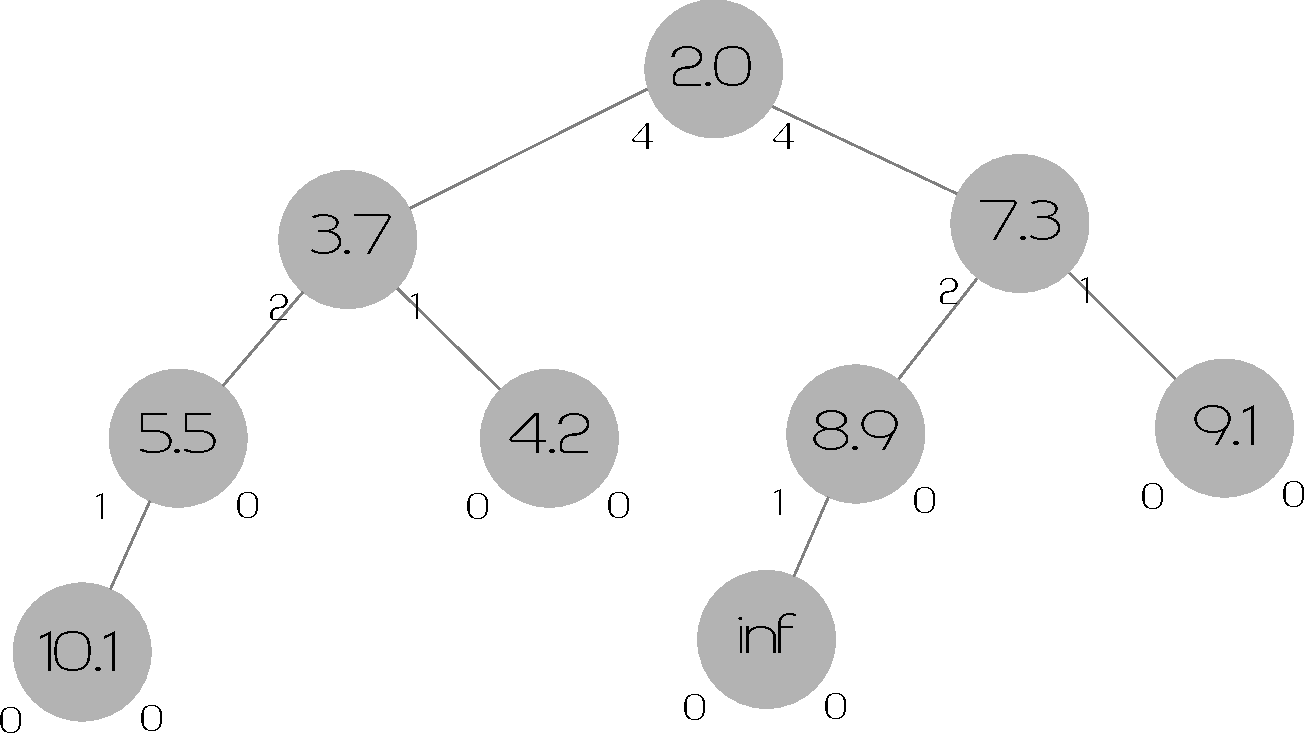
\includegraphics[width=0.99\textwidth]{img/extipq.pdf}
    \caption{Indexed Priority Queue extended with descendant count per branch}
    \label{img:ipq}
  \end{center}
\end{figure}

Our idea is, for each node, to keep track of the number of descendant per branch, having in such way the possibility to keep the tree balanced when adding nodes. In figure \ref{img:ipq} we show how the same IPQ drawn in \cite{gibson2000} would appear with our extension. Given this data structure, the procedures to add and remove a new node \texttt{n} are described respectively in \Cref{algo:newnode} and \Cref{algo:remnode}, in which the procedure \texttt{UPDATE\_AUX(n)} is the same described in \cite{gibson2000}.

\begin{algorithm}
\begin{distribalgo}[1]
\vspace{5pt}
\IF{root does not exist}
  \STATE{\texttt{n} is the new root}
\ELSE
  \STATE{\texttt{c} $\gets$ root}
  \WHILE{\texttt{c} has two descendants}
    \IF{\texttt{c.right} $<$ \texttt{c.left}}
      \STATE{\texttt{dir} $\gets$ right}
    \ELSE
      \STATE{\texttt{dir} $\gets$ left}
    \ENDIF
    \STATE{add $1$ to count of \texttt{dir} descendants}
    \STATE{\texttt{c} $\gets$ \texttt{c.dir}}
    \IF{\texttt{c} has not the left child}
      \STATE{\texttt{n} becomes left child of \texttt{c}}
      \STATE{set count of left nodes of \texttt{c} to $1$}
    \ELSE
      \STATE{\texttt{n} becomes right child of \texttt{c}}
      \STATE{set count of right nodes of \texttt{c} to $1$}
    \ENDIF
  \ENDWHILE
  \STATE{\texttt{UPDATE\_AUX(n)}}
\ENDIF
\caption{Procedure to add a new node \texttt{n}}
\label{algo:newnode}
\end{distribalgo}
\end{algorithm}

\begin{algorithm}
\begin{distribalgo}[1]
\vspace{5pt}
\STATE{\texttt{c} $\gets$ root}
\WHILE{\texttt{c} is not a leaf}
  \IF{\texttt{c.left} $>$ \texttt{c.right}}
    \STATE{\texttt{dir} $\gets$ left}
  \ELSE
    \STATE{\texttt{dir} $\gets$ right}
  \ENDIF
  \STATE{subtract $1$ to count of \texttt{dir} descendants}
  \STATE{\texttt{c} $\gets$ \texttt{c.dir}}
\ENDWHILE
\IF{\texttt{c} $\neq$ \texttt{n}}
  \STATE{swap \texttt{n} and \texttt{c}}
  \STATE{remove \texttt{n}}
  \STATE{\texttt{UPDATE\_AUX(c)}}
\ELSE
  \STATE{remove \texttt{n}}
\ENDIF
\caption{Procedure to remove a node \texttt{n}}
\label{algo:remnode}
\end{distribalgo}
\end{algorithm}

Using the two procedures described above, the topology of the whole tree is constrained to remain balanced despite the dynamic addition and removal of reactions.

\section{Meta-meta model}
\label{meta-meta-model}
The complexity of the systems we want to design is achieved by the following set of common key properties:
\begin{itemize}
 \item situatedness -- they deal with spatially- and possibly socially-situated activities of entities, and should therefore be able to interact with a limited portion of the surrounding world and contextualise their behaviour accordingly; 
 \item adaptivity -- they should inherently exhibit properties of autonomous adaptation and management to survive contingencies without external intervention, global supervision, or both; 
 \item self-organisation -- spatial and temporal patterns of behaviour should emerge out of local interactions and without a central authority that imposes pre-defined plans.
\end{itemize}

Among the many natural metaphors one can use as inspiration for modelling and developing artificial systems with the above properties \cite{ecosystems-jpcc7}, we consider chemistry following a series of work in the field of pervasive computing \cite{VCMZ-TAAS2011,VZ-INS2010,sapere-procedia7}. 
%
We argue that there are three main issues to be resolved in order to build a meta-model that can be sufficiently expressive for our purpose starting from a purely chemical model:
\begin{enumerate}
 \item the concept of environment where agents are situated and can move is missing in a model that considers only intercommunicating chemical compartments;
 \item the only available mean for changing the system status is the execution of a reaction;
 \item the only data item that chemical reactions can manipulate are molecules' concentrations, namely numbers connected to a particular token.
\end{enumerate}

In the following discussion, we will use interchangeably compartment/agent/node and reaction/events as synonyms.
%
As first step, we introduce the environment, absent in chemistry-derived SSAs, as first class abstraction.
%
The environment has responsibility to provide, for each compartment, a set of compartments that are its neighbours.
%
The rule which is applied to determine whether or not a node belongs to another node's neighbourhood  can be arbitrarily complicated.
%
Also, it is responsible of exposing possible physical boundaries, namely, to limit the possible movements of compartments situated within the environment.

The fact that reactions are the only abstraction the modeller can rely upon in order to let the simulated system progress is not a difficult problem by itself.
%
In fact, nothing prevents to widen the generality of a reaction by defining it as: ``a set of conditions that, when matched, trigger a set of actions on the environment''.

With this definition in mind, a condition is a function that associates to each possible state of the environment a numeric value ranging from zero to positive infinity.
%
If such value is zero, the event can not be scheduled; otherwise, it is up to the reaction to interpret the number: it can influence or not the time at which the reaction will be scheduled, depending on the specific reaction implementation.
%
In case we desire to re-build the original chemical model, we would define a condition for each of the molecules on the left-hand side of the chemical reaction that return the number of molecules currently available in the local compartment.
%
Also, we would define the reaction in such a way that it correctly interprets the number returned by the conditions as concentration of each reactant and correctly applies the rules for computing a propensity to be used to influence the reaction speed \cite{gillespie1977}.

In this framework, actions are arbitrary changes of the environment.
%
In case of pure chemistry, the actions of a reaction would be one for each reactant (that must be removed from the local compartment) and one for each product (that must be added to the local compartment).
%
In case of an extended model considering also multiple compartments, an action should be programmed to be responsible of transferring molecules from a node to a neighbouring one.

Both conditions and actions must expose the set of possible data items (molecules) that they may read or modify: this is necessary in order to allow the dependency graph to be built.
%
Also, both conditions and actions must expose a context of the type \localc{}, \neighborhood{} or \globalc{}; it will be used internally to determine the input and output contexts for the reaction itself.

The reactions are responsible of computing their expected execution time.
%
The engine may require such putative time to be updated in two cases: i) the reaction has just been executed or ii) a reaction on which this reaction depends on has been executed.
%
In case of update required, the reaction should leverage a separately defined time distribution to compute the next putative execution time, possibly feeding the time distribution with a summary of the data gathered from conditions.
%
In case of a Poisson process, a negative exponential time distribution initialised with $\lambda{} = r$ should be used, for instance.
%
In case of a repetitive event, such as a timer, a Dirac comb may be used.

In this model the atomicity of the reactions represent a double edged sword: on the one hand, they allow for arbitrarily complex behaviours to be ordered and executed within a DES, on the other hand they make it difficult to model events that last in time, e.g. to simulate devices with limited computational power on which some complex task takes a not negligible amount of time to get completed.
%
To support something similar, two reactions should be defined: one to trigger the start of the computation, and another to actually run it and complete.

The low expressive power of the classical concentration is probably the hardest challenge to tackle when trying to extend a chemical-born meta model towards a richer world, where data items can be complex structures and not just simple numbers.
%
We have found no trivial solution to this issue; instead, we propose to make the definition ``concentration'' depend on the actual meta-model: let ``concentration'' be ``the data items agents can manipulate''.
%
Besides the trivial example of chemistry, where data items are integer numbers, let's consider a distributed tuple spaces model: in this case, the molecules would be tuples, and the concentration would be defined as ``the set of tuples matching a certain tuple''.
%
Clearly, such flexibility comes with a cost: since the conditions and actions operating on different concentrations dramatically change their behaviour, for any possible class of data items the meta-model must be instanced with a proper set of conditions and actions that can act on such ``concentration''.
%
We call this set of concentration-specific instances of conditions and actions an ``incarnation''.
%
This sort of model inheritance justifies our double ``meta'' level: the model described is a meta-meta-model, an incarnation is a meta-model, and, finally, a specific scenario instancing one of such meta-models is a model.

\label{model}
\begin{figure}%[H]
  \begin{center}
    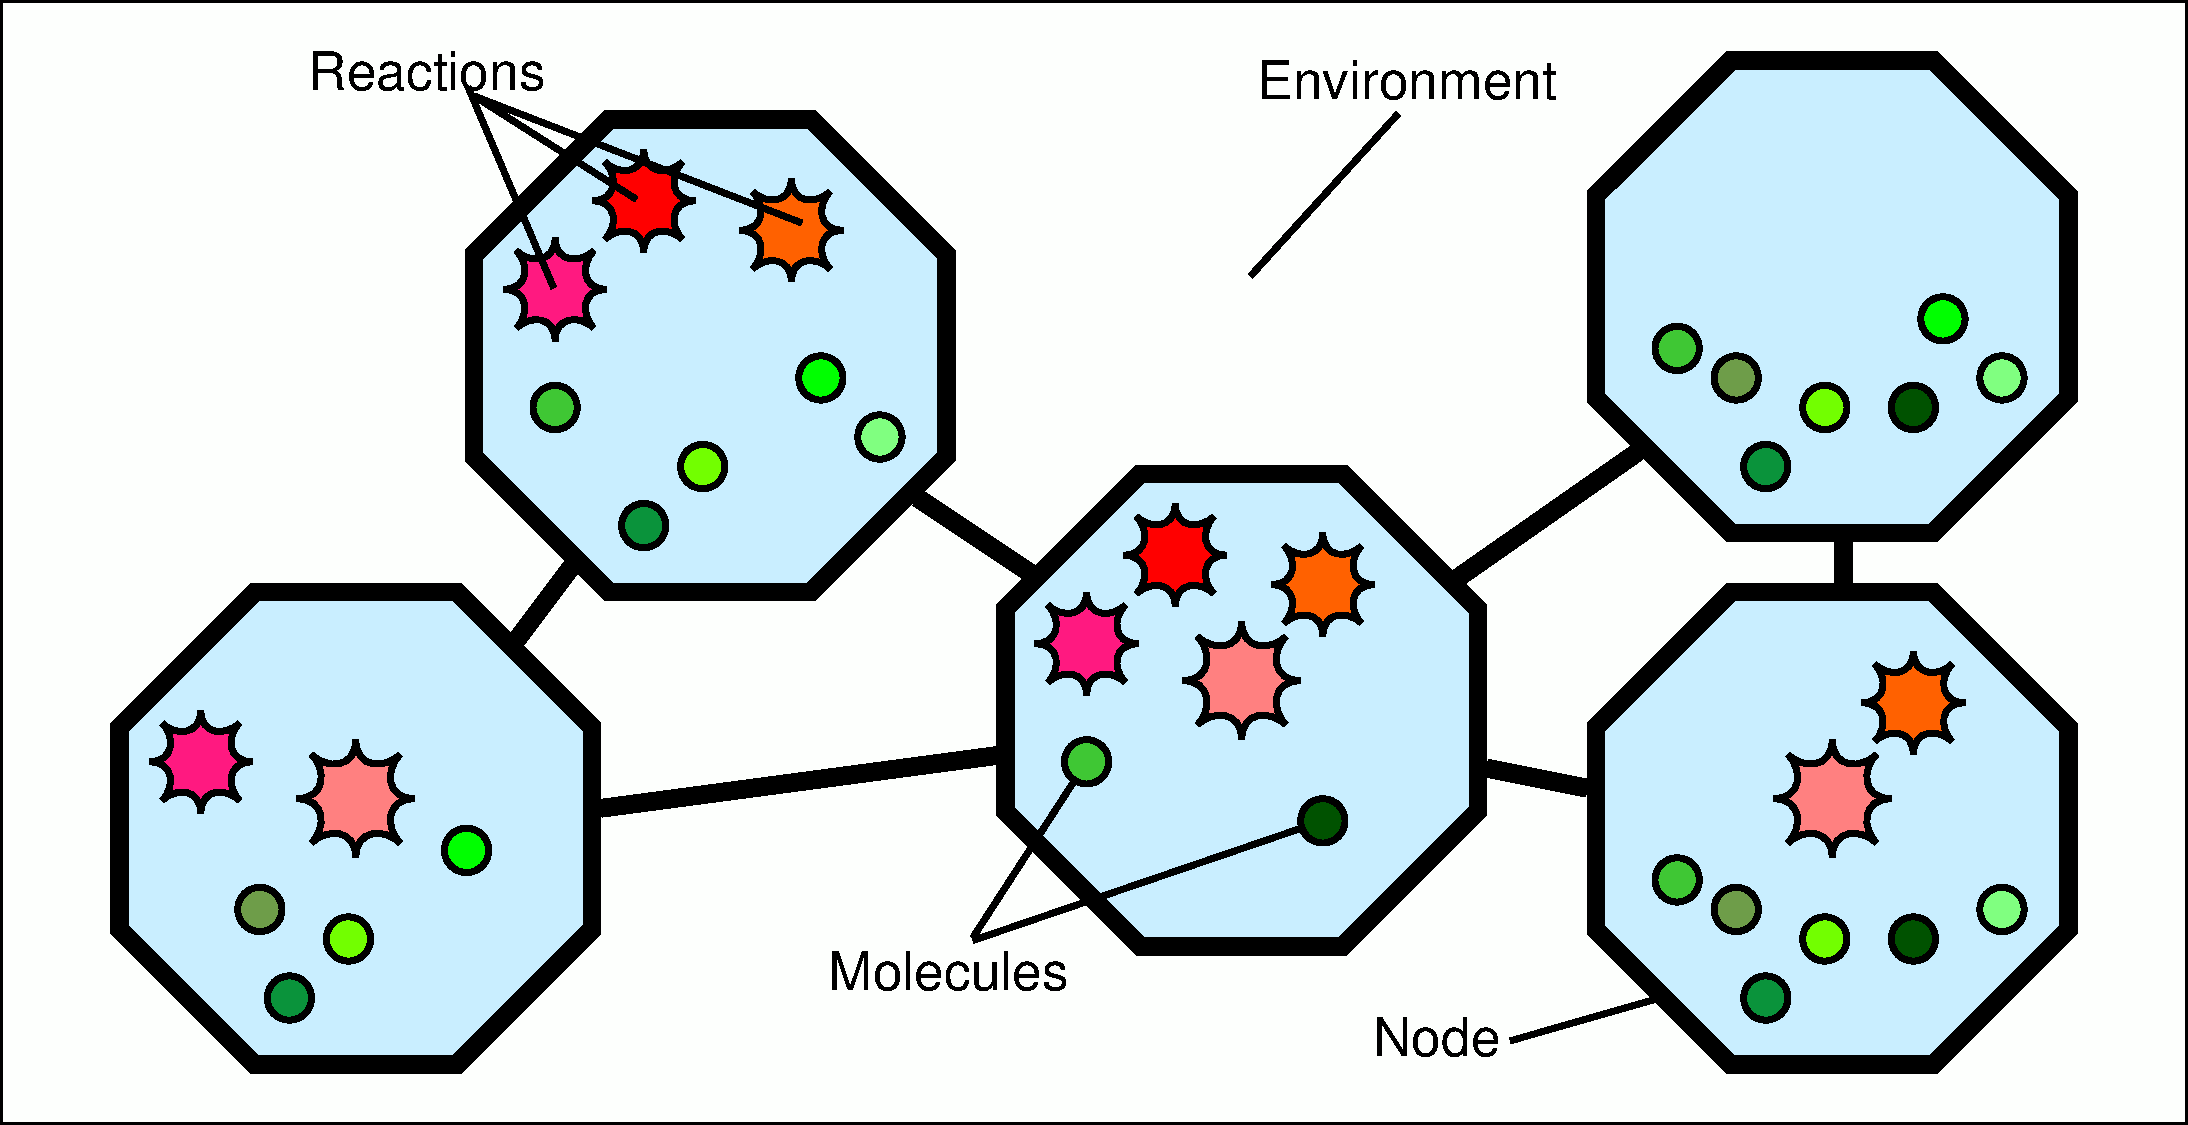
\includegraphics[width=0.99\columnwidth]{img/model.pdf}
    \caption{\alchemist{} computational model: it features a possibly continuous space embedding a linking rule and containing nodes. Each node is programmed with a set of reactions and contains a set of structured molecules.}
    \label{img:model}
  \end{center}
\end{figure}

A pictorial representation of the underlying meta-meta-model is shown in \Cref{img:model}.
%
In this vision of the world, an environment is a multi dimensional space, continuous or discrete, which is able to contain nodes and which is responsible of linking them following a rule.
%
The environment may or not allow nodes to move.
%
Nodes are entities which can be programmed with a set of reactions, possibly changing over time.
%
They also contain molecules, each one equipped with a data structure generalising on the concept of ``concentration''.

\begin{figure*}%[H]
  \begin{center}
    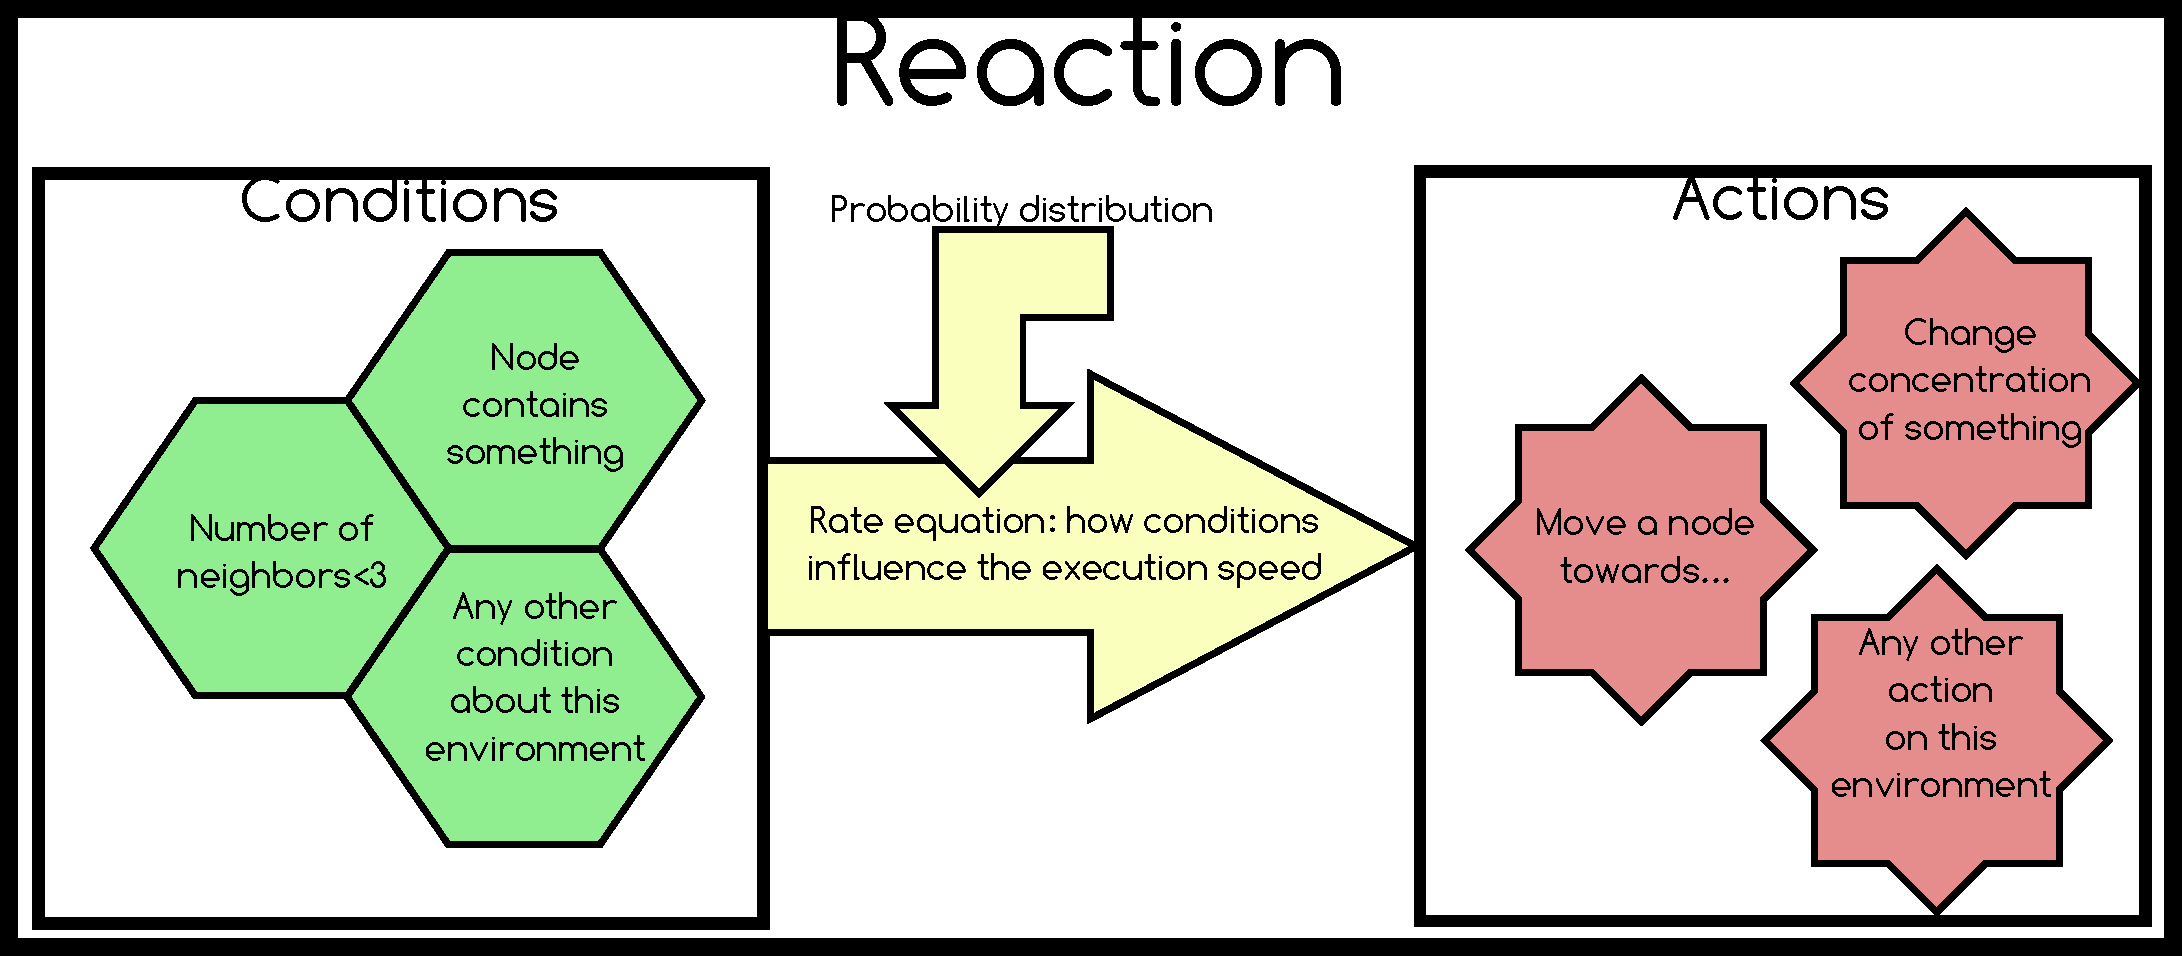
\includegraphics[width=0.99\textwidth]{img/reaction.pdf}
    \caption{\alchemist{} model of reaction: a set of conditions on the environment that determines whether the reaction is executable, a rate equation describing how the speed of the reaction changes in response to environment modifications, a probability distribution for the event and a set of actions, which will be the neat effect of the execution of the reaction.}
    \label{img:reaction}
  \end{center}
\end{figure*}

The concept of reaction is graphically depicted in \Cref{img:reaction}.
%
It allows, for example, to model reactions which are faster if a node has many neighbours, or also reactions that resemble complex biological phenomena such as the diffusion of morphogenes during embryo development as described in \cite{LeccaJIB2010}.
%
It also allows to define which kind of time distribution to use to trigger reactions: this enables us to model and simulate systems based on Continuous Time Markov Chains (CTMCs), to add triggers, or also to rely just on classical discrete time ``ticks''.


\section{Architecture}
%TODO: architettura da rifare

\label{subsec:architecture}
\begin{figure}%[H]
  \begin{center}
    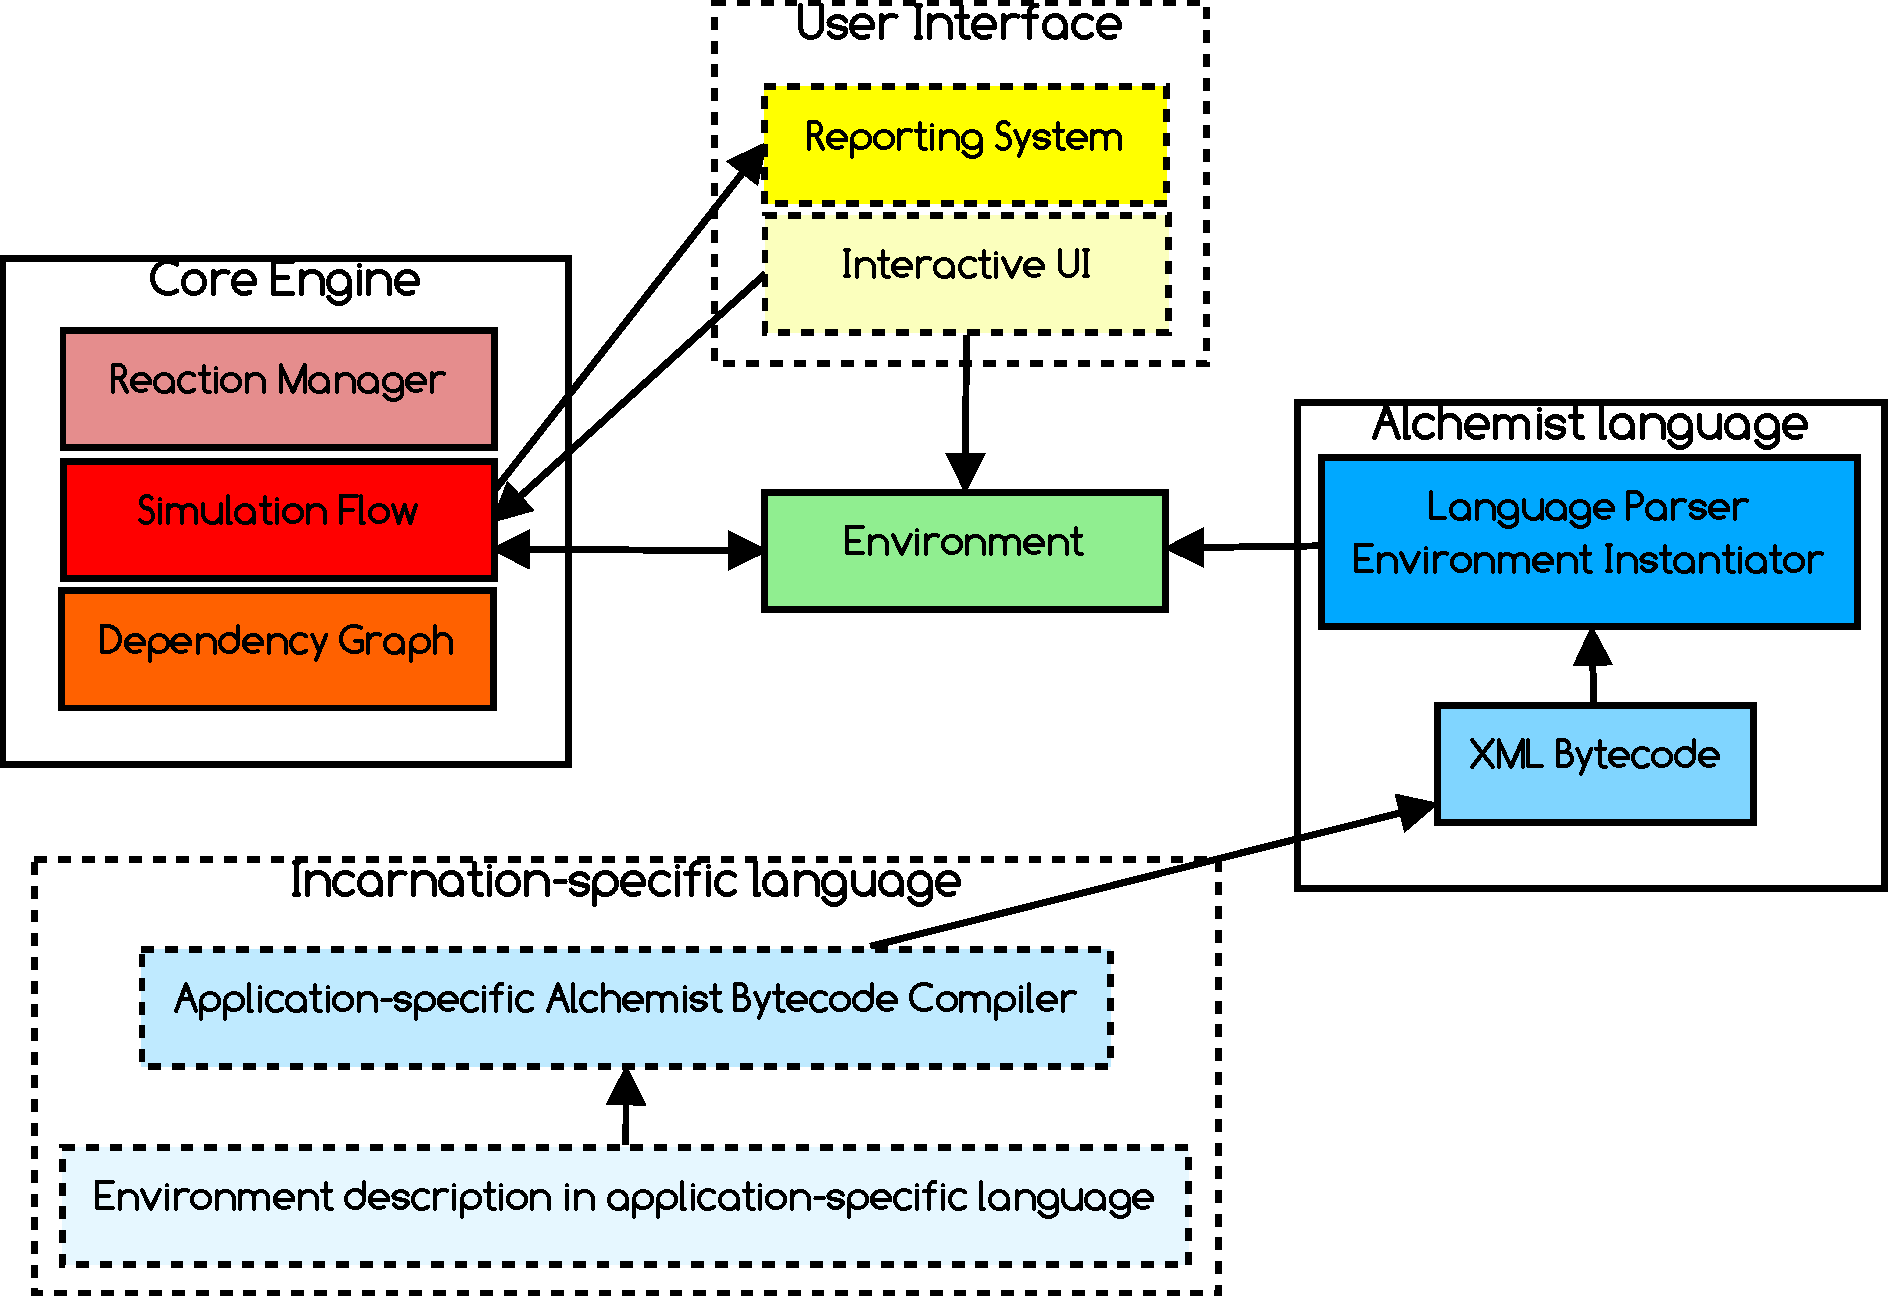
\includegraphics[width=0.99\columnwidth]{img/structure.pdf}
    \caption{\alchemist{} architecture. Elements drawn with continuous lines indicates components common for every scenario and already developed, those with dotted lines are extension-specific components which have to be developed with a specific incarnation in mind.}
    \label{img:arch}
  \end{center}
\end{figure}

The whole framework has been designed to be fully modular and extensible.
The whole engine or parts of it can be re-implemented without touching anything in the model, and on the other hand the model can be extended and modified without affecting the engine.

It is important to note that there is no restriction about the kind of data structure representing the concentration, which can in fact be used to model structured information: by defining a new kind of structure for the concentration, it is possible to incarnate the simulator for different specific uses. For example, by assessing that the concentration is an integer number, representing the number of molecules currently present in a node, \alchemist{} becomes a stochastic simulator for chemistry. A more complex example can be the definition of concentration as a tuple set, and the definition of molecule as tuple template. If we adopt this vision, \alchemist{} can be a simulator for a network of tuple spaces. Each time a new definition of concentration and molecule is made, a new ``incarnation'' of \alchemist{} is automatically defined. For each incarnation, a set of specific actions, conditions, reactions and nodes can be defined, and all the entities already defined for a more generic concentration type can be reused.


%TODO: scrivere una ncarnazione e poi magari anche scrivere una simulazione.

\subsection{Writing a simulation}

%SISTEMARE%

In order to write a simulation, the user must have, or implement herself, an incarnation of \alchemist{}, as described in \Cref{subsec:architecture}.

As shown in \Cref{img:arch}, the simulations are written in a specific XML language containing a complete description of environment and reactions. This code is interpreted in order to produce an instance of an environment: once it is created, no further interpretation is needed in order to run the simulation. This XML code is not meant to be directly exploited by users, but it represents a way of describing environments in a machine-friendly format and is a formalisation of the generic model of \alchemist{}. The idea behind this choice is that \alchemist{} is flexible enough to be used in various contexts, each one requiring a personalised language and a different instantiation of the model. It is up to the extensor to write a translation module from its personalised language to the \alchemist{} XML. Of course, it is also possible to code the simulation behaviour  directly with Java.

\subsection{Implementation details}
%TODO%
The framework was developed from scratch using Java. Being performance a critical issue for simulators, we compared some common languages in order to evaluate their performance level.
%
Surprisingly, Java performance are at same level of compiled languages such as C/C++ \cite{bull2003, oancea2011}.
%
The Java language was consequently chosen because of the excellent trade off between performance, easy portability and maintainability of the code, and the high-level support for concurrent programming at the language level. 
%
The COLT Java library\footnote{\url{http://acs.lbl.gov/software/colt/}} provided us the mathematical functions we needed.
%
In particular, it offers a fast and reliable random number generation algorithm, the so called Mersenne Twister \cite{matsumoto1998}.

% TODO! %
\alchemist{} is still actively developed and currently consists of about 200 classes for about 20'000 lines of code. Though still in beta version, it is released with GPL license as open source \footnote{\mbox{\url{http://alchemist.apice.unibo.it}}.}.

\section{Performance}
\begin{figure}[t]
    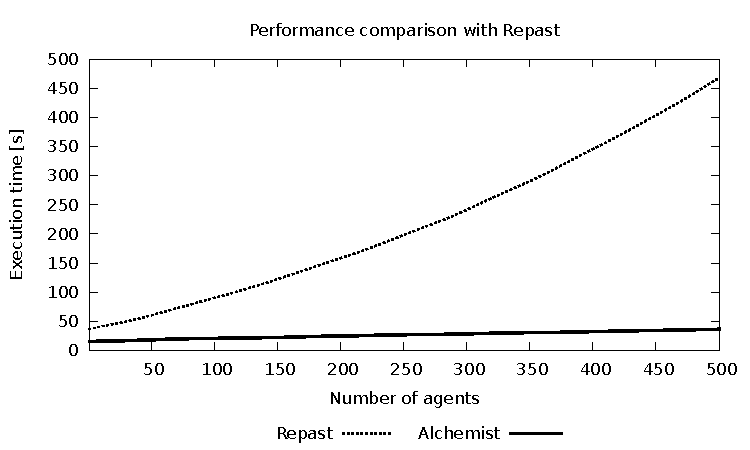
\includegraphics[width=0.999999\columnwidth]{img/jos-graph01}
    \caption{Chart showing the performance scaling of \alchemist{}}
    \label{img:repastperf}
\end{figure}

It is possible to evaluate and compare the performances of \alchemist{} with respect to some known MABS.
%
We exemplify it considering Repast, which we used to developed an alternative simulation for the case study presented in \Cref{jos-museum}\footnote{The source code of the simulation we developed is publicly available at \mbox{\url{http://apice.unibo.it/xwiki/bin/view/Alchemist/JOS/}.}}. There are some important facts that deserve discussion here.

First, since there is no built-in support for stochastic simulation in Repast, we choose to collapse the last five laws of \Cref{img:museum-rules} into a single code path, and the same was made for \alchemist{} by defining a new action.
%
In that way, we were able to avoid for this very specific case the need of a full fledged dependency graph, because there will always be exactly one \textbf{source} and one \textbf{field} per sensor, and no reactions need to be enabled or disabled.
%
This crippled most of the effectiveness of \alchemist{}'s dependency graph, which is indeed a source of optimisation not natively existing in Repast---developing a dependency graph for stochastic simulation in Repast is out of the scope of this thesis, though it would be an interesting subject for future work.
%
On the other hand, it would have been unfair to compare our optimised version against just a plain Gillespie's algorithm built upon Repast.

The second important point is that we choose to encode all the data in both Repast and \alchemist{} as an array of double values instead of real tuples.
%
For \alchemist{}, this meant that we developed a new incarnation for the precise scope of this performance test.
%
The choice of encoding data that way made things faster (no matching required), but also less general.
%
This was done because the SAPERE incarnation of \alchemist{}, which allows us to write the laws as in \Cref{img:museum-rules}, requires a matching system that is not easily portable to Repast.

We choose the configuration of \Cref{img:museum-generalmap2} and we run multiple simulations varying the number of agents per group, in order to evaluate how the two systems scale with the problem size.
%
We measured the running time required to our testbed to run the simulation from the time zero to the time 100.
%
No graphical interface were attached to the simulators while running the batch, in order to evaluate only the raw performance of the engine.
%
The system we used was an Intel Core i5-2500 equipped with 8GB RAM, with Sabayon Linux 7 as operating system and Sun Java HotSpot\texttrademark{} 64-Bit Server version 1.6.0\_26-b03 as Java Virtual Machine.
%
Results are shown in \Cref{img:repastperf}.

Results show the simulator built upon the \alchemist{} framework to be at least twice faster and to scale better than the one built on Repast.
%
Being the dependency graph optimisation cut off as explained above, the reasons for such a difference can lay on the internal scheduler of the engine or in the optimisations in the model.
%
For the first point, we used the default scheduler of Repast Symphony, which is a binary heap implemented through a plain Java array, while our implementation relies on the algorithm and data structures already presented in \Cref{chemical-engine}, so there is not a substantial efficiency difference.
%
For the latter point, a big difference in terms of performances is due to the heavy optimizations of the neighbourhoods of the default \alchemist{} continuous environment.
%
Since the concept of neighbourhood was part of the computational model, it was possible to adopt caching strategies in order to ensure a fast access to the neighbourhood and a quick execution of the operations on it.
%
This is probably the component which gives the highest impact in this case, since most interactions occur among an agent and its neighbourhood.



\section{Collocation in literature}

\subsection{\alchemist{} as a DES}

\alchemist{} is a discrete event simulator (DES), since it combines a continuous time base with the description of system dynamics by distinguished state changes \cite{Zeigler2000}.
%
Since it allows for in-simulation modifications of the environment, it can be considered to belong to the fourth generation of DESs according to \cite{BabulakIJOE2008}.
%
The work in \cite{Pollacia89} surveys the classical DES approaches: according to it, \alchemist{} belongs to the category of simulators featuring ``internal clock'', ``next-event time advance'', and adhering to the ``Event-scheduling World View'', namely, the simulator handles events and is concerned with their effect on system states.

Apart from the meta-model adopted, the main innovative aspect of \alchemist{} with respect to the general DES approach is its ability of optimising the ``compile current event list'' stage \cite{Pollacia89}, which \alchemist{} quickly executes incrementally by means of the management of dependencies that the adoption of a chemical-like model enables.

As far as the simulator model is concerned, instead, the class of DES more related to our approach are those commonly used to simulate biological-like systems.
%
A recent overview of them is available in \cite{EwaldJOS2007}, which takes into account: DEVS \cite{zeigler1984}, Petri Nets \cite{murata1989}, State Charts \cite{Harel1987} and stochastic $\pi$-calculus \cite{Priami1995}.
%
Such an overview however emphasises that all such models require a considerable effort to map biological components into abstractions of the chosen formalism: this is because none of them was specifically developed with biology or bio-inspiration in mind.
%
As described in \Cref{meta-meta-model}, our model is meant to overcome such limitations, since all the enhancements to the basic chemical model we support can be seen as a generalisation of the abstractions of the works presented in \cite{EwaldJOS2007}, and add to them the possibly of customising with much greater flexibility a simulation to the scenarios of bio-inspired computational systems.

We should finally note that the DES approach typically contrasts the use of mathematical techniques (e.g. modelling the system by differential equations).
%
However, the possible different choice of translating a system model to ordinary or partial different equations -- which can be solved numerically in a time considerably shorter than a set of stochastic simulations -- is shown to be impractical in our case.
%
This path, explored for example by \cite{MallavarapuInterface2008}, can provide good results for dynamics that progress at more or less the same speed, and in which abundance of species (data-items or agents in our case) is so high that it can be relaxed to real-valued variables \cite{EwaldJOS2007}.
%
This is not the case for many scenarios even in system biology (see, for example, \cite{Cowan2000, UhrmacherWSC2005}), not to mention scenarios like pervasive computing where reaction rates do not change continuously, and where the effect on an even small number of agents can be key to a given system evolution.

\subsection{\alchemist{} as a MABS}

Even though chemical-inspired, the meta-meta-model described in \Cref{meta-meta-model} holds evident relationships with multi-agent-based simulation (MABS) approaches.

According to \cite{BandiniJASSS2009}, agent-based platforms for simulations can be split in three categories: general purpose frameworks with specific languages (such as NetLogo), general purpose frameworks based on general purpose programming languages (such as Repast \cite{repast}) and frameworks which provide an higher level linguistic support, often targeted to a very specific application (e.g. \cite{WeynsAAMAS2006}).
%
Each approach has clearly its own advantages and weaknesses.
%
Usually, the more general purpose is the language, the wider is the set of possible scenarios, and the wider is also the gap between the language and the simulated model.
%
This means that an higher level language allows the user to create and tune its simulations in an easier way, on the other hand it often restricts the generality of the tool. 

\alchemist{} is meant to provide a set of meta-models, possibly each with its own domain specific language, still maintaining the possibility to extend or re-implement certain abstractions using the general purpose Java language (defining a new ``incarnation'', namely a new meta-model).

\subsubsection{Advantages}

There is a set of applications which are better tackled by \alchemist{}.
%
In particular, \alchemist{} is suitable for all those simulation scenarios in which agents have relatively simple behaviour, and the notion of agent-based environment plays instead a fundamental role in organising and regulating the agents' activities \cite{BandiniE4MAS2006} by both enabling local interactions among the proactive entities \cite{HellebooghAAMAS2007} and enforcing coordination rules \cite{aose-mags5}, allowing the modeller to shift her focus from the local behaviour of the single agent to a more objective vision of the whole MAS \cite{SchumacherCEEMAS2007}. 
%
The idea of dealing with a strong notion of environment in multi-agent systems has been deeply developed in a series of work: other than its importance in the simulation context \cite{HellebooghAAMAS2007}, at the infrastructure level \cite{VHRSZ-JAAMAS2007} and at the methodological level \cite{aose-mags5}, there have been proposals of meta-models such as A\&A \cite{artifacts-jaamas17} and infrastructures such as {\sf TuCSoN} \cite{tucson-aamas99} and {\sc CArtAgO} \cite{RPV-JAAMAS2011}.
%
A common viewpoint of all these works is that the behaviour of those passive and reactive components structuring the environment (e.g. \emph{artifacts} in A\&A) is well defined in terms of rules expressed as declarative conditions-imply-actions fashion.
%
Accordingly, \alchemist{} is particularly useful either in computing systems following the chemical inspiration \cite{VCMZ-TAAS2011,VZ-INS2010,sapere-procedia7}, or for agent-oriented systems where the role of the environment is key, up to be a very dynamic part of the whole system---where network nodes (or, in biological terms, compartments) can move, new nodes can be spawn or be removed from the system, and links can appear or break at runtime as happen e.g. in pervasive computing scenarios \cite{sapere-procedia7}.

\subsubsection{Limitations}

Inevitably, as an attempt to build a hybrid between agent-based simulators and (bio)chemical simulators, some trade-offs had to be accepted, which ultimately makes \alchemist{} less suited for certain classes of applications.
%
In particular, a limitation is that \alchemist{}'s agent actions have to be mapped onto the concept of reaction. 
%
On the one hand, this makes it rather straightforward to create reactive memoryless agents \cite{BandiniJASSS2009}, whose goal is just to perform rather easy computations resulting in the creation, deletion or modification of information items in the environment.
%
In fact, since it is allowed to program different nodes with different reactions, it is easy to code reactive and context-dependent agents. On the other hand, there is neither out-of-the-box facility nor any high level abstraction useful to define intelligent agents \cite{BandiniJASSS2009}. The simulator is able to run them provided the user manually writes their whole behaviour as a single Java-written reaction---and properly specifies dependencies with other reactions.
%
Although possible in principle, performing this task too frequently is likely breaking the \alchemist{} abstraction, making the programmer losing the nice declarative approach that chemistry endorses, and possibly hampering the optimisation techniques that motivated \alchemist{}.

\section{Chemical meta-model}
\subsection{Example scenario: Morphogenesis}
\section{SAPERE meta-model}
\subsection{Example scenario: Crowd Steering}
\label{jos-museum}
In this section, we show the SAPERE meta-model at work in the framework in a crowd steering case study in which a middleware has the goal of leading people in the desired location within a complex environment in short time, avoiding obstacles such as crowded regions and without global supervisioning. 

Consider a museum with a  set of rooms, whose floor is covered with a network of computational devices (infrastructure nodes). These devices can exchange information with each other based on proximity, sense the presence of visitors, and hold information about expositions currently active in the museum. Each room has four exits and they are connected via external corridors. Visitors wandering the museum are equipped with a hand-held device that holds the visitor's preferences. By interaction with infrastructure nodes, a visitor can be guided towards rooms with a target matching their interest, thanks to signs dynamically appearing on his smartphone or on public displays. This is done using techniques suggested in the field of spatial computing \cite{VCMZ-TAAS2011}---namely, computational gradients injected in a source and diffusing around such that each node holds the minimum distance value from the source.

The environment is a continuous bidimensional space with walls. 
%
Smartphones (or public displays) are agents dynamically linked with the nearest infrastructure node -- the neighbours are the sensors inside a certain radius $r$, parameter of the model -- from which they can retrieve data in order to suggest visitors where to go. Visitors are agents which follow the advices of their hand-held device (or public displays). It is defined a minimum possible distance between them, so as to model the physical limit and the fact that two visitors can't be in the same place at the same time. Visitors can move of fixed size steps inside the environment. If an obstacle is on their path, their movement is shortened to the allowed position nearest to the desired place.

All the information exchanged is in form of annotations, simply modelled as tuples $\lsa{v_1,\ldots,v_n}$ (ordered sequence) of typed values, which could be for example numbers, strings, structured types, or function names.
%
\noindent There are three forms of annotations used in this scenario:

{\[\begin{array}{l}
 \lsa{\mathtt{source}, id, type, N_{max}} \\
 \lsa{\mathtt{field}, id, type, value, tstamp} \\
\lsa{\mathtt{info}, id, crowd, M, t'} \\
\end{array}\]}

\noindent A \textbf{source} annotation is used as a source with the goal of generating a field: $id$ labels the source so as to distinguish sources of the same type; $type$ indicates the type of fields in order to distinguish different expositions; $N_{max}$ is the field's maximum value. 
%
A \textbf{field} annotation is used for individual values in a gradient: $value$ indicates the individual value; the $tstamp$ reflects the time of creation of the annotation; the other parameters are like in the source annotation.
%
An \textbf{info} annotation is supposed to be created and kept up to date by each sensor. $M$ represents the number of smartphones the sensor is perceiving as neighbours.

The rules are expressed in form of chemical-resembling laws, working over patterns of annotations.
%
One such pattern $P$ is basically an annotation which may have some variable in place of one or more arguments of a tuple, and an annotation $L$ is matched to the pattern $P$ if there exists a substitution of variables which applied to $P$ gives $L$.
%
A law is hence of the kind \mbox{$P_1,\ldots,P_n\xmapsto{r}P'_1,\ldots,P'_m$}, where: \emph{(i)} the left-hand side (reagents) specifies patterns that should match annotations $L_1,\ldots,L_n$ to be extracted from the local annotation space; \emph{(ii)} the right-hand side (products) specifies patterns of annotations which are accordingly to be inserted back in the space (after applying substitutions found when extracting reagents, as in standard logic-based rule approaches); and \emph{(iii)} rate $r$ is a numerical positive value indicating the average frequency at which the law is to be fired---namely, we model execution of the law as a CTMC transition with Markovian rate (average frequency) $r$. If no rate is given the reaction is meant to be executed ``as soon as possible'', which means that the rate that associated with the reaction tends to infinite.
%
To allow interaction between different nodes (hence, annotation spaces), we introduce the concept of \emph{remote pattern}, written $\rem{P}$, which is a pattern that will be matched with an annotation occurring in a neighbouring space.
\begin{figure*}
{\footnotesize\[\begin{array}{rcl}

 \lsa{\mathtt{source}, id, type, N_{max}}  &  \xmapsto{r_{\mathit{init}}} &  \lsa{\mathtt{source}, id, type, N_{max}}, \lsa{\mathtt{field}, id, type, N_{max}, \#T}  \\

 & & \\

 \lsa{\mathtt{field}, id, type, N,  t} & \xmapsto{r_{\mathit{diff}}} &  \lsa{\mathtt{field}, id, type, N, t}, \rem{\lsa{\mathtt{pre\_field}, id, type, N-\#D, t}} \\
 
  & & \\
 
\lsa{\mathtt{pre\_field}, id, type, N, t}, \lsa{\mathtt{info}, id, crowd, M, t'} & \xmapsto{} &  \lsa{\mathtt{field}, id, type, N-k*C, t},\lsa{\mathtt{info}, id, crowd, M, t'} \\

 & & \\

\lsa{\mathtt{field}, id, type, N, t}, \lsa{\mathtt{field}, id, type, M, t' +t} & \xmapsto{} & \lsa{\mathtt{field}, id, type, M, t'+t}\\

 & & \\

\lsa{\mathtt{field}, id, type, N, t}, \lsa{\mathtt{field}, id, type, M, t} &\xmapsto{} & \lsa{\mathtt{field}, id, type, max(M,N),  t}\\
  
 & & \\

\lsa{\mathtt{field}, id, type, N, t}, \lsa{\mathtt{field}, id', type, N+M, t'} & \xmapsto{} & \lsa{\mathtt{field}, id', type, N+M, t'}\\
  

 & & \\

\end{array}\]}
%$}
\caption{Laws describing the museum application.}
\label{img:museum-rules}
\end{figure*}

As sources annotations are injected in nodes, gradients are built by the first three rules in \Cref{img:museum-rules}. 
%
The first one, given a source, initiates the field with its possible maximum value. 
%
The second one, when a node contains a field annotation, spreads a copy of it to a neighbouring node picked up randomly with a new value computed considering the crowding around the sensor. The parameter $k$ allows to tune how much crowding should influence the field, while $\#D$ is the measure of the distance between the two involved sensors. 
%
% The third eco-law, when a node contains a pre\_field LSA of type $type$ and a field LSA of type $type'$ by which the pre\_field depends, removes the pre\_field LSA and creates a new field LSA with a value computed according to the transformation function,  $\mu$, which elaborates the values $N$ and $M$ of the two reactants. 
%This is done by removing the pre-field LSA and by adding the field LSA with the new value. 
% The purpose of this law is to model the interactions between fields. For instance we may assume that if there is a crowd which jams a region of the museum, that path towards the target should have less probability of being picked, so the value of the target field has to be reduced. 
%
As a consequence of these laws, each node will carry a field annotation indicating the topological distance from the source. The closest is the field value to $N_{max}$, the nearest is the field source. When the spread values reach the minimum value $0$, the gradient has to become a plateau.

To address the dynamism of the scenario where people move, targets being possibly shifted, and crowds forming and dissolving, we introduced the following mechanism.
%
We expect that if a gradient source moves the diffused value has to change according to the new position. 
%
This is the purpose of the $tstamp$ parameter which is used in the fourth law, continuously updating old values by more recent ones (\emph{youngest} law).
%
In this way we ensure that the system is able to adapt to changes of the source states. 
%
Finally, the spreading law above will produce duplicate values in locations, due to multiple sources of the same type (indicated by different ids), multiple paths to a source, or even diffusion of multiple annotations over time. For this reason we introduced the last two laws. They retain only the maximum value, i.e. the minimum distance, the former when there are two identical annotations with only a different value, the latter when the id is different (\emph{shortest} laws).
%
The proposed solution is  intrinsically able to dynamically adapt to unexpected events (like node failures, network isolation, crowd formation, and so on) while maintaining its functionality.

People are modelled as nodes programmed with a single reaction with no conditions and having, as action, the ability to follow the highest field value among neighbouring sensors.
%
For the crowding annotation, we may assume that sensors are calibrated so as to locally inject and periodically update it by setting the current level of crowding, \emph{i.e.} the number of persons.
%
The reaction rates are identified by hand performing different simulations with different parameters. The results reported are obtained with $r_{init} = 1$ and $r_{diff} = 50$. The other laws show no rate because it is assumed to be infinite (as-soon-as-possible semantics).

\subsubsection{Simulation Results}

\begin{figure*}[t]
\begin{center}
    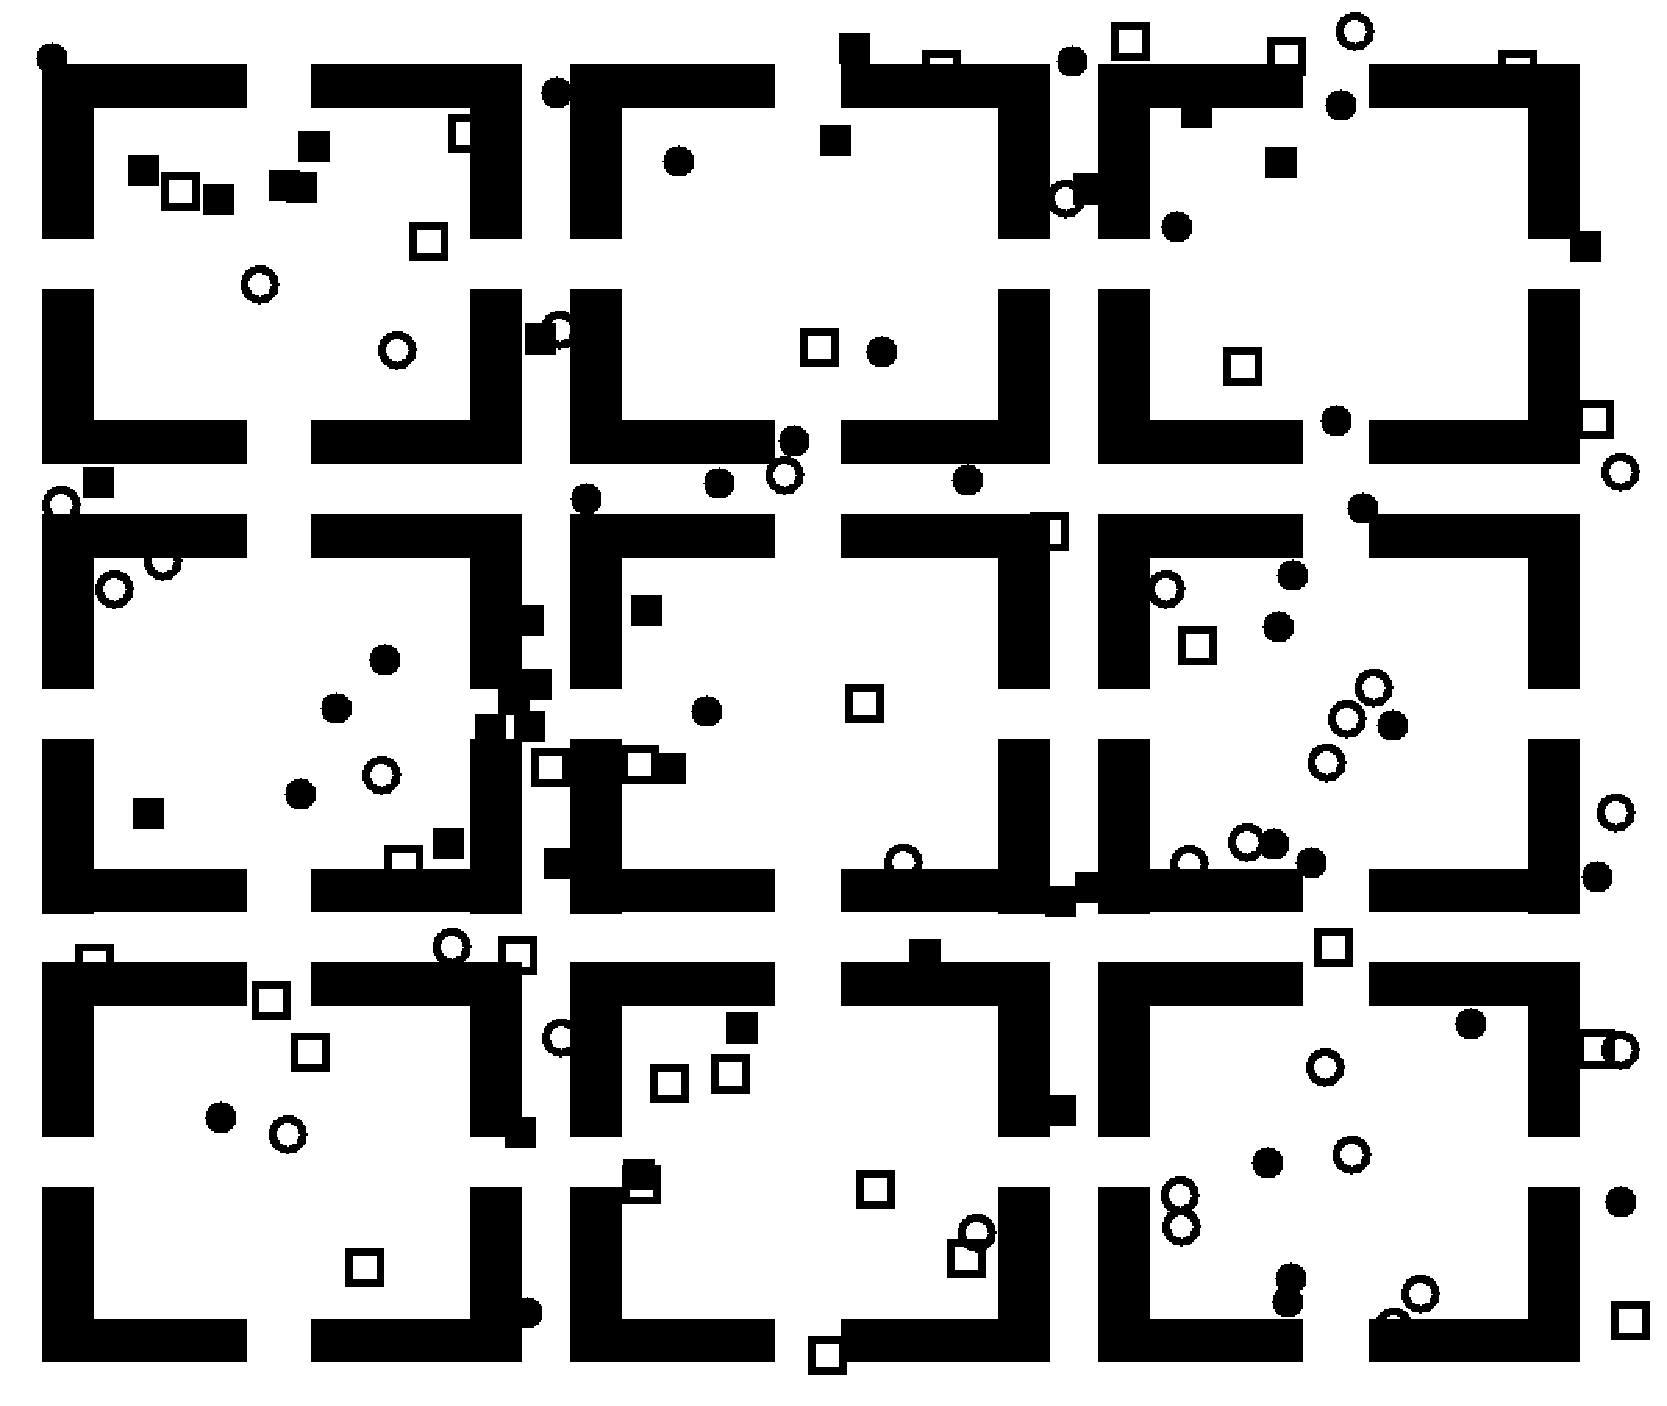
\includegraphics[width=0.3\columnwidth]{img/jos-snapshots/4-1}
    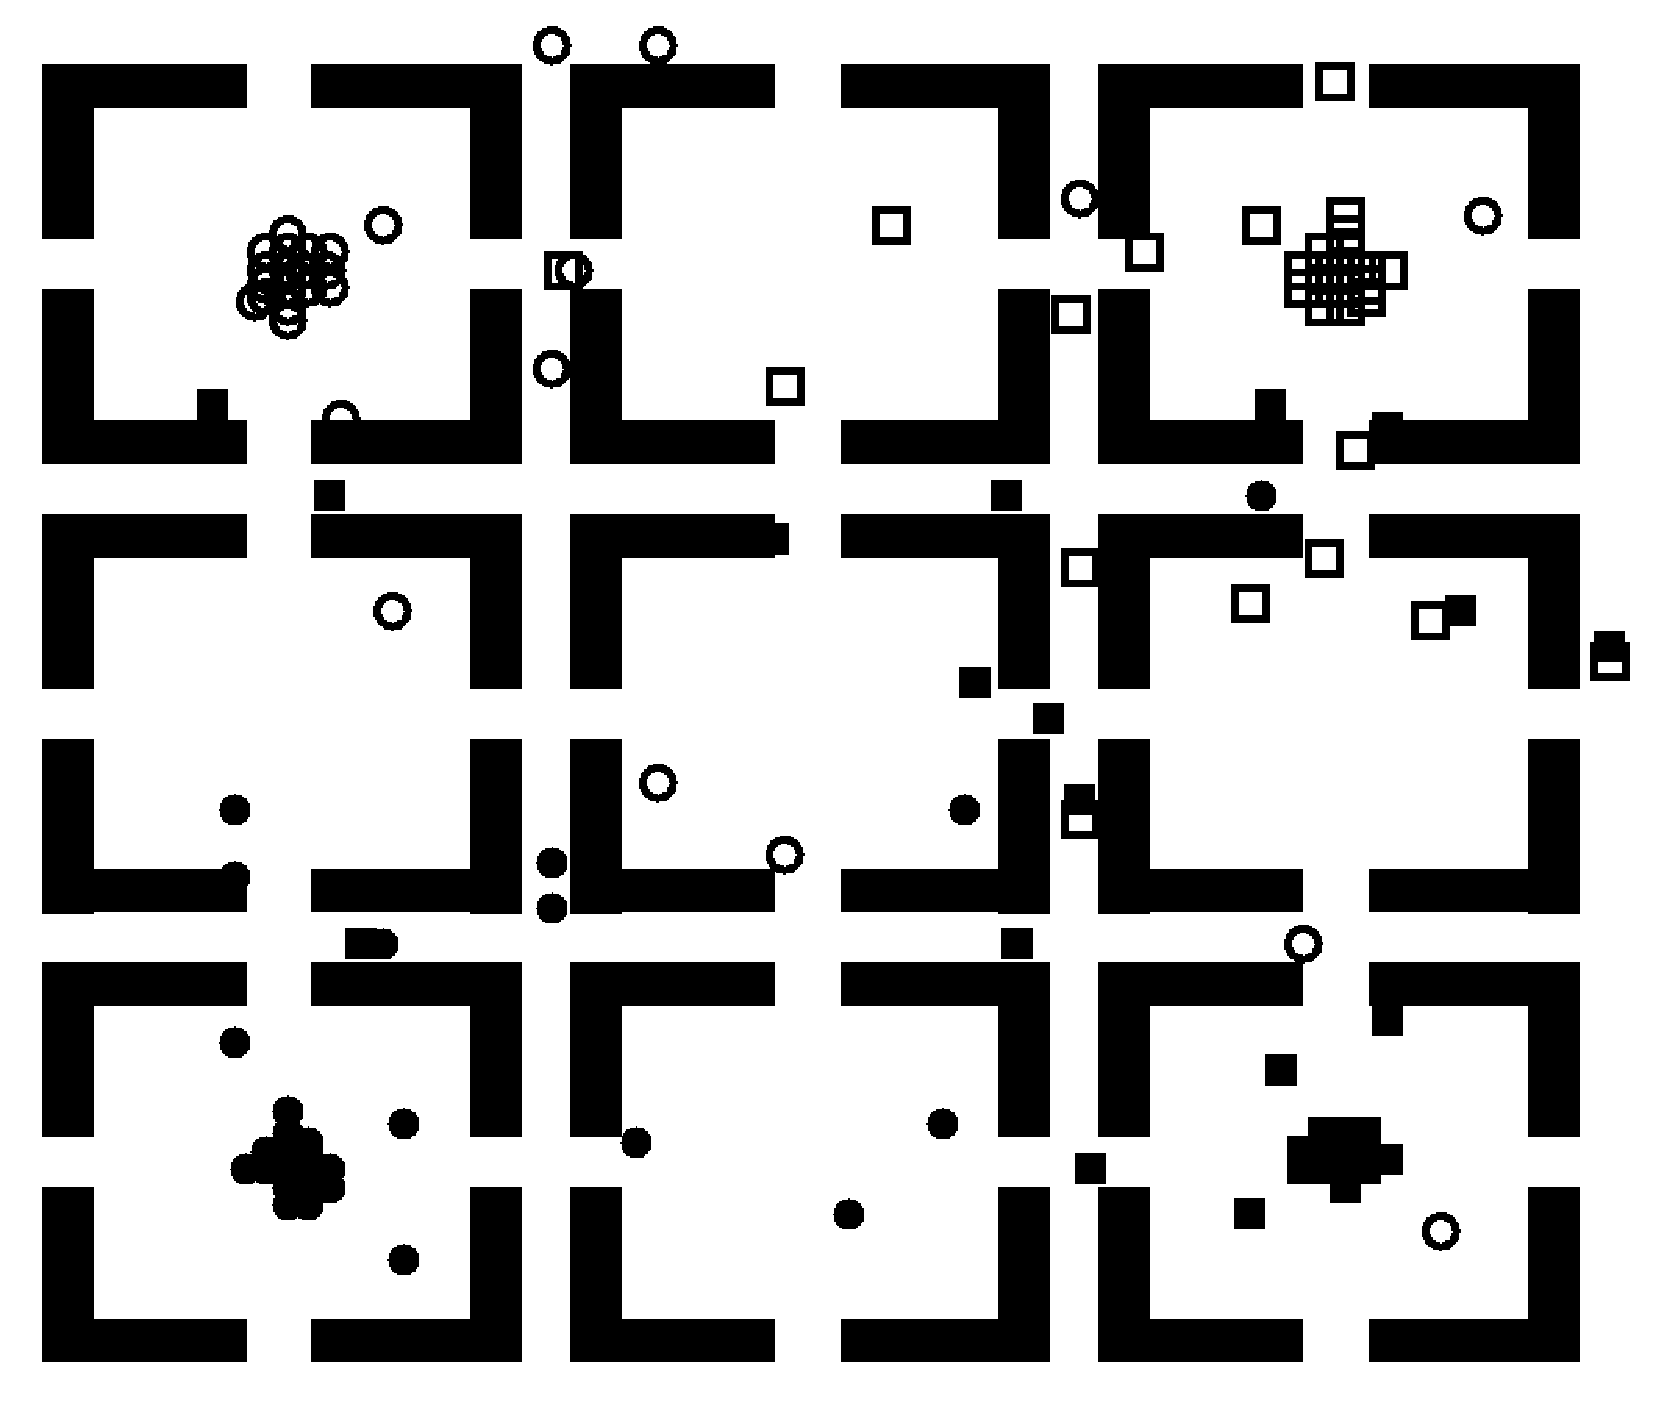
\includegraphics[width=0.3\columnwidth]{img/jos-snapshots/4-3}
    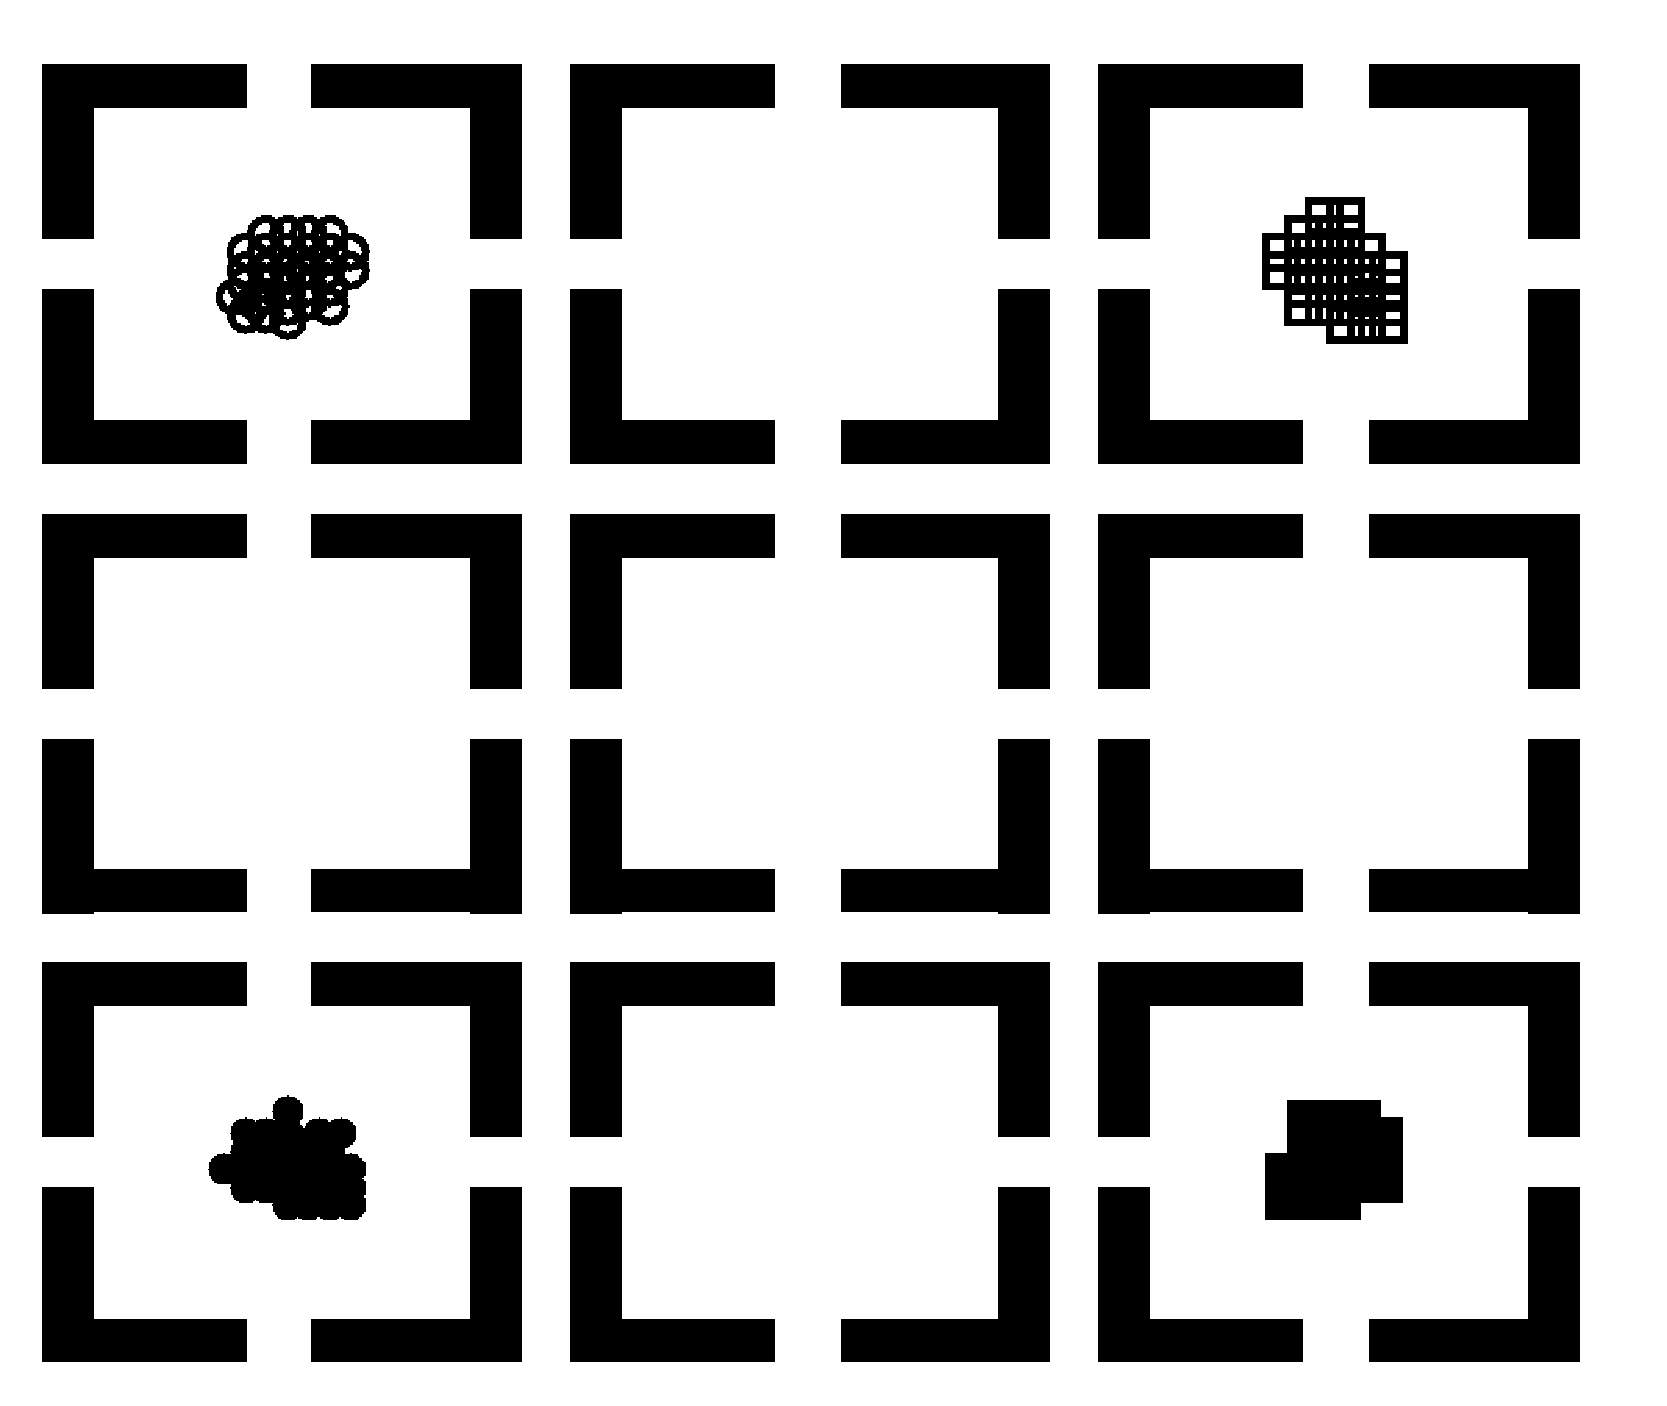
\includegraphics[width=0.3\columnwidth]{img/jos-snapshots/4-4}
    \caption{A simulation run of the reference exposition: three snapshots of \alchemist{}'s graphic reporting module with this simulation. \label{img:museum-generalmap}}    
\end{center}
\end{figure*}

We here present simulations conducted over an exposition, where nine rooms are connected via corridors. 
%
People can express different preferences represented by their shape.

Three snapshots of a first simulation run are reported in \Cref{img:museum-generalmap}. 
%
We here consider four different targets that are located in the four rooms near environment angles.
%
People are initially spread randomly in the museum, as shown in the first snapshot, and they eventually reach the room in which the desired target is hosted, as shown in the last snapshot. 


\Cref{img:museum-generalmap2} shows a simulation experimenting with the effect of crowding in the movement of people.
%
Two groups of people -- denoted with empty and full circles -- with common interests are initially located in two different rooms, as shown in the first snapshot. 
%
The target for the dark visitors is located in the central room of the second row, while the others' is in the right room of the second row.
%
In the simulation, dark visitors reach their target soon because it is nearer, thus forming a crowded area intersecting the shortest path towards the target for the other visitors.
%
Due to this jam the latter visitors choose a different path that is longer but less crowded. 

\begin{figure*}[t]
\begin{center}
    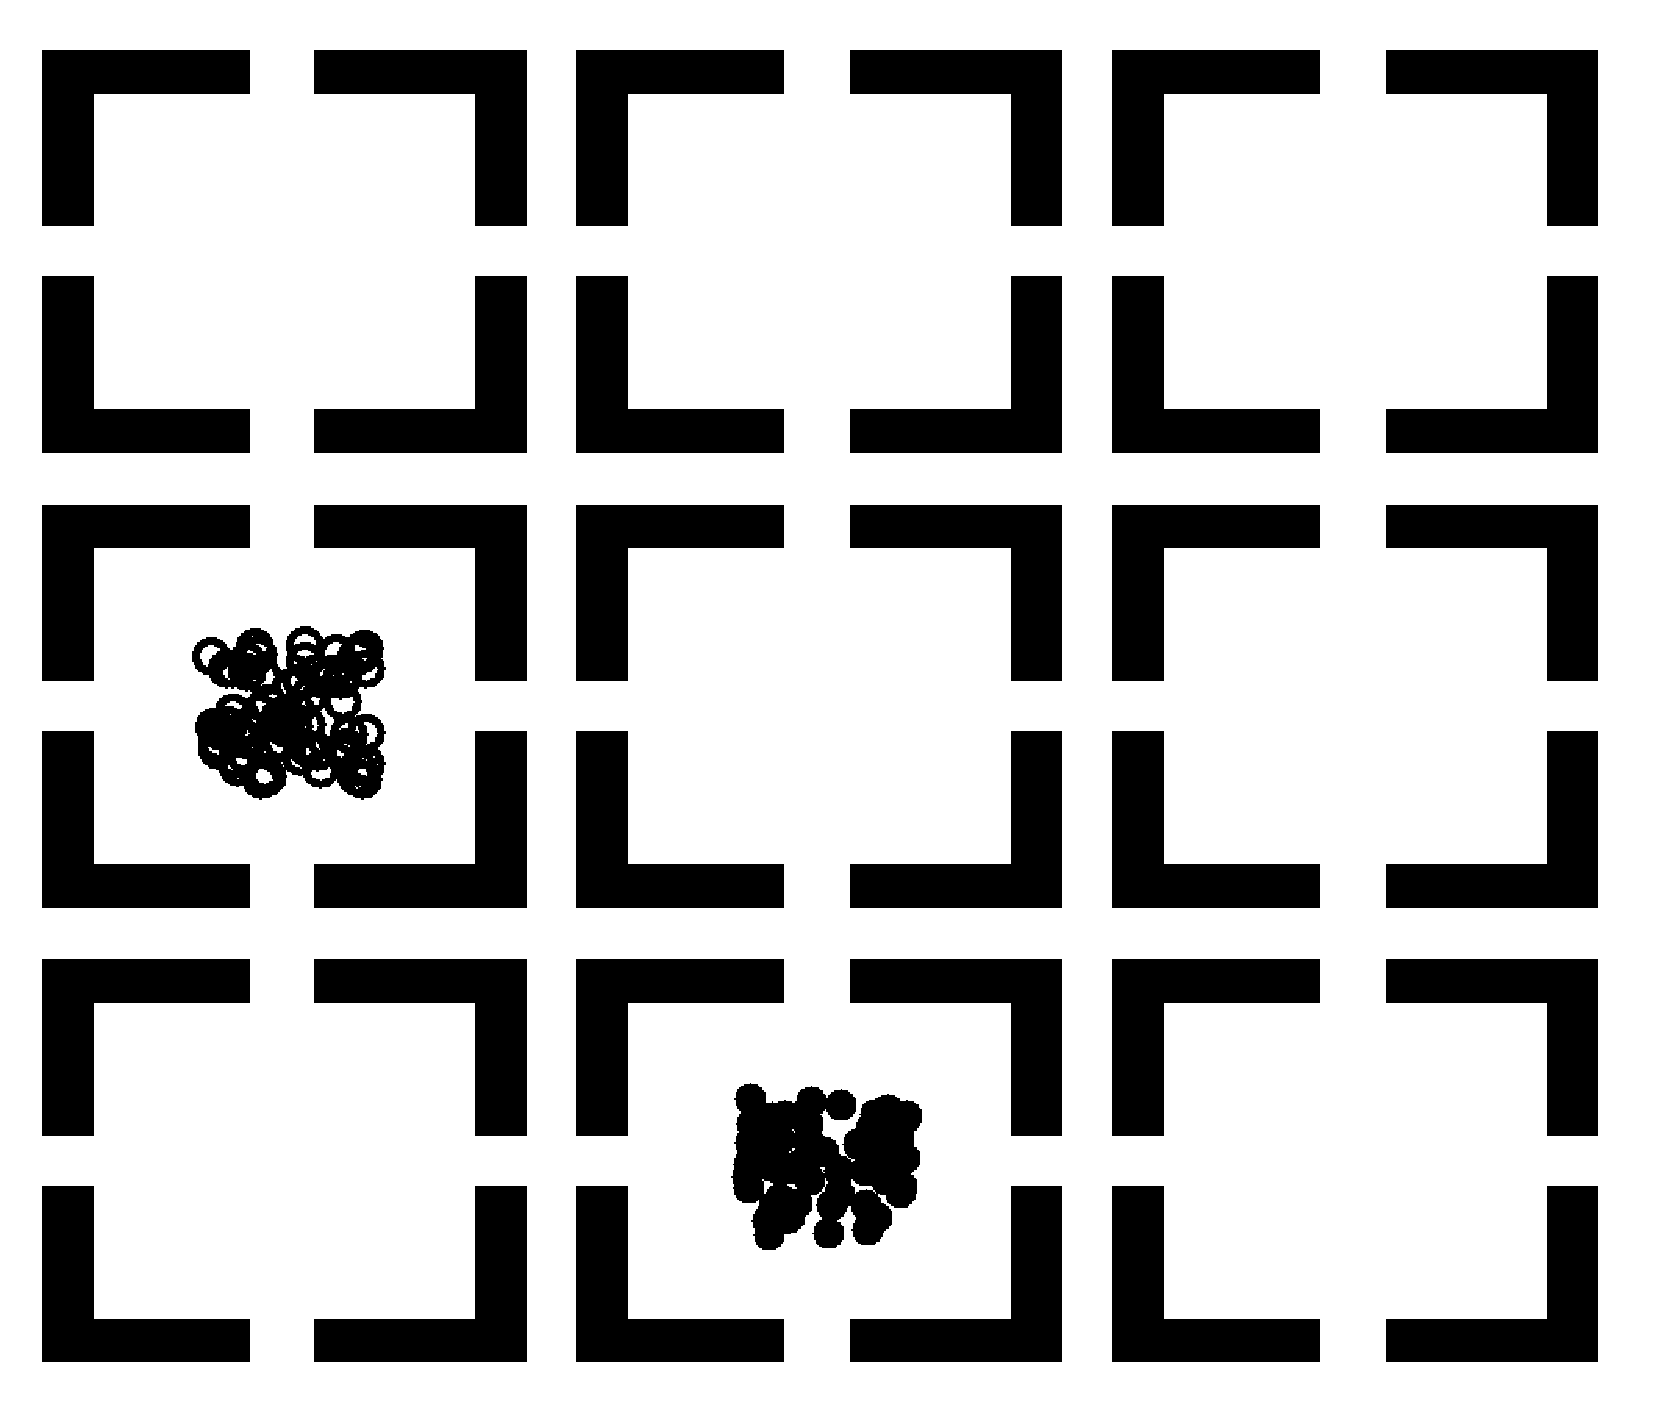
\includegraphics[width=0.3\columnwidth]{img/jos-snapshots/2-1}
    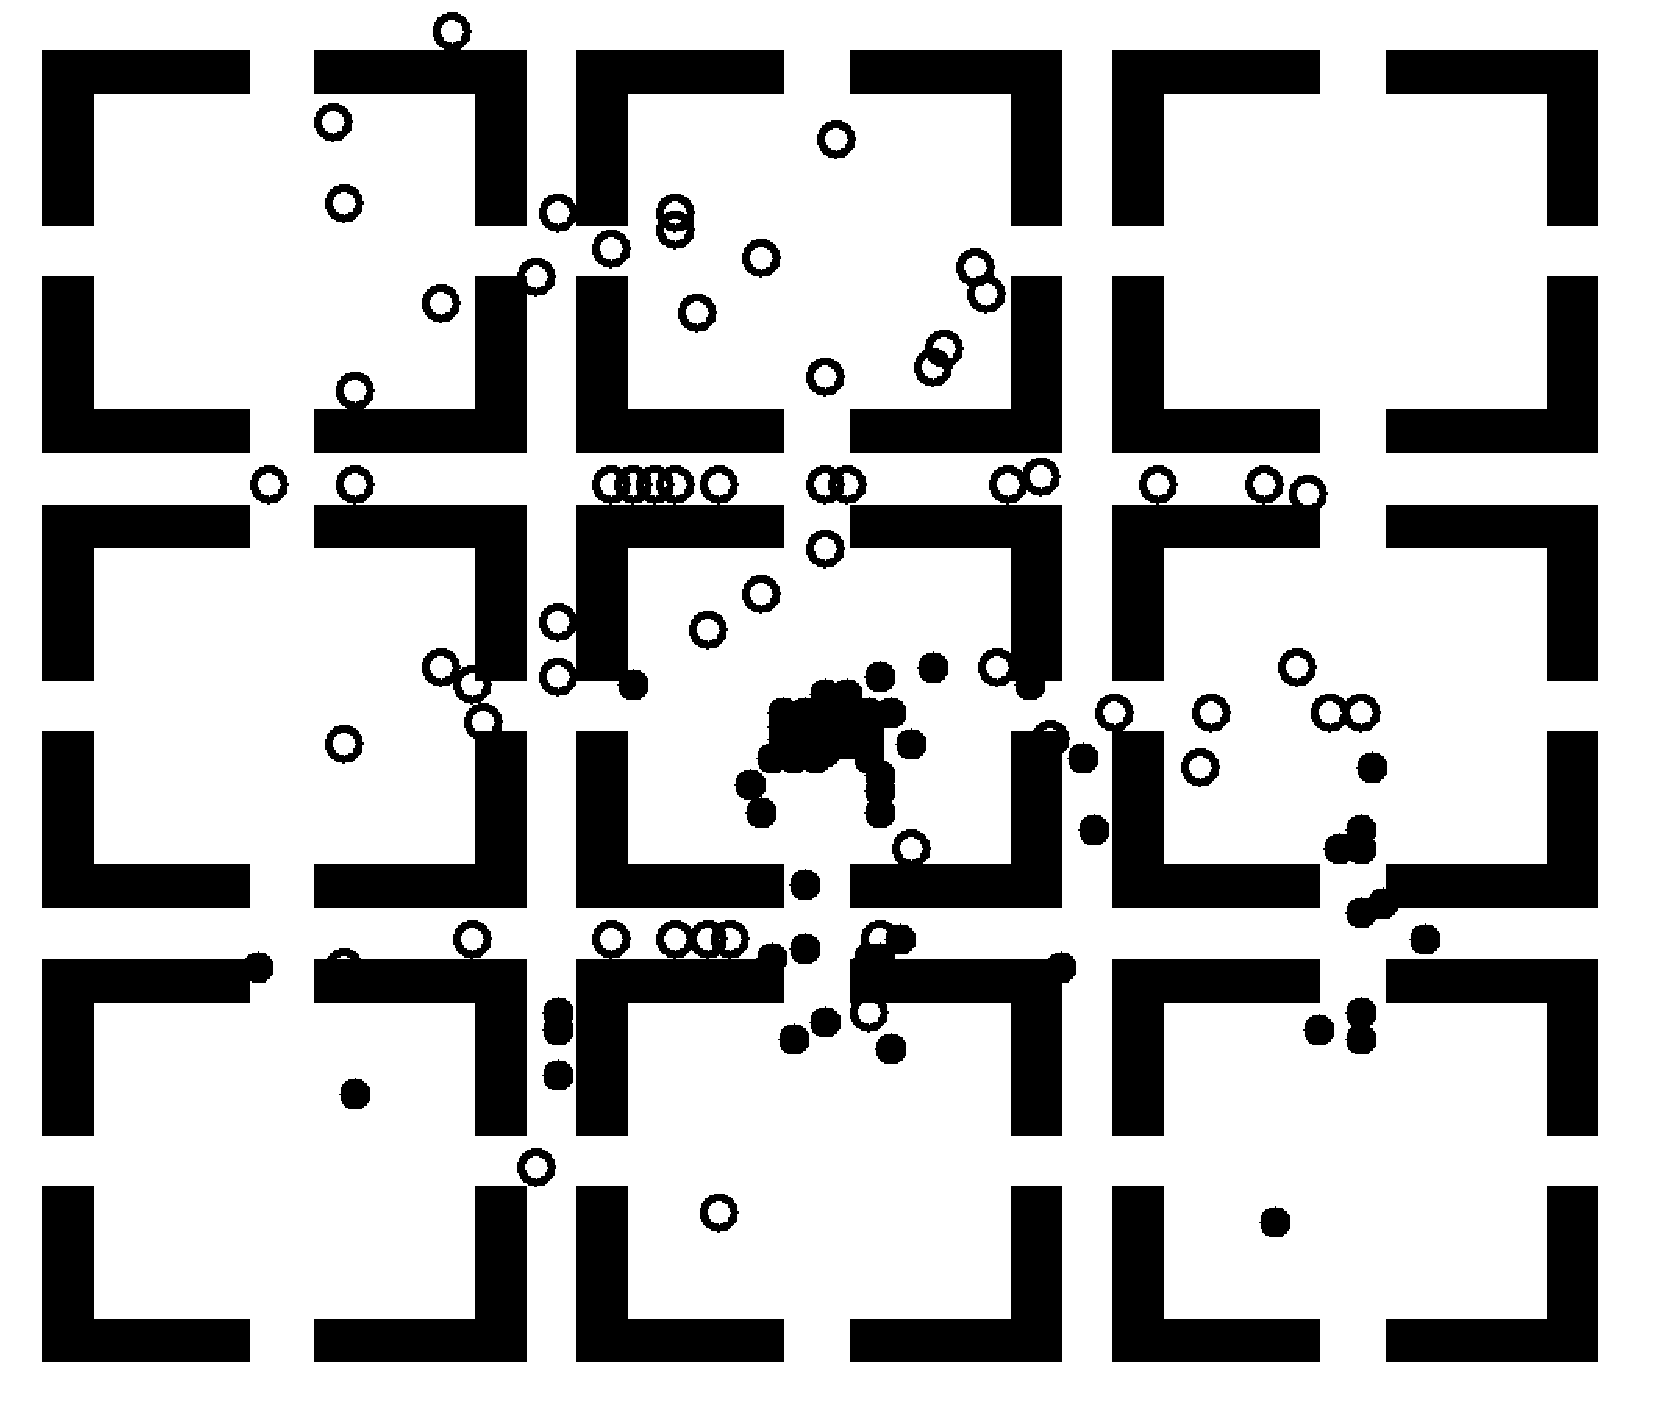
\includegraphics[width=0.3\columnwidth]{img/jos-snapshots/2-3}
    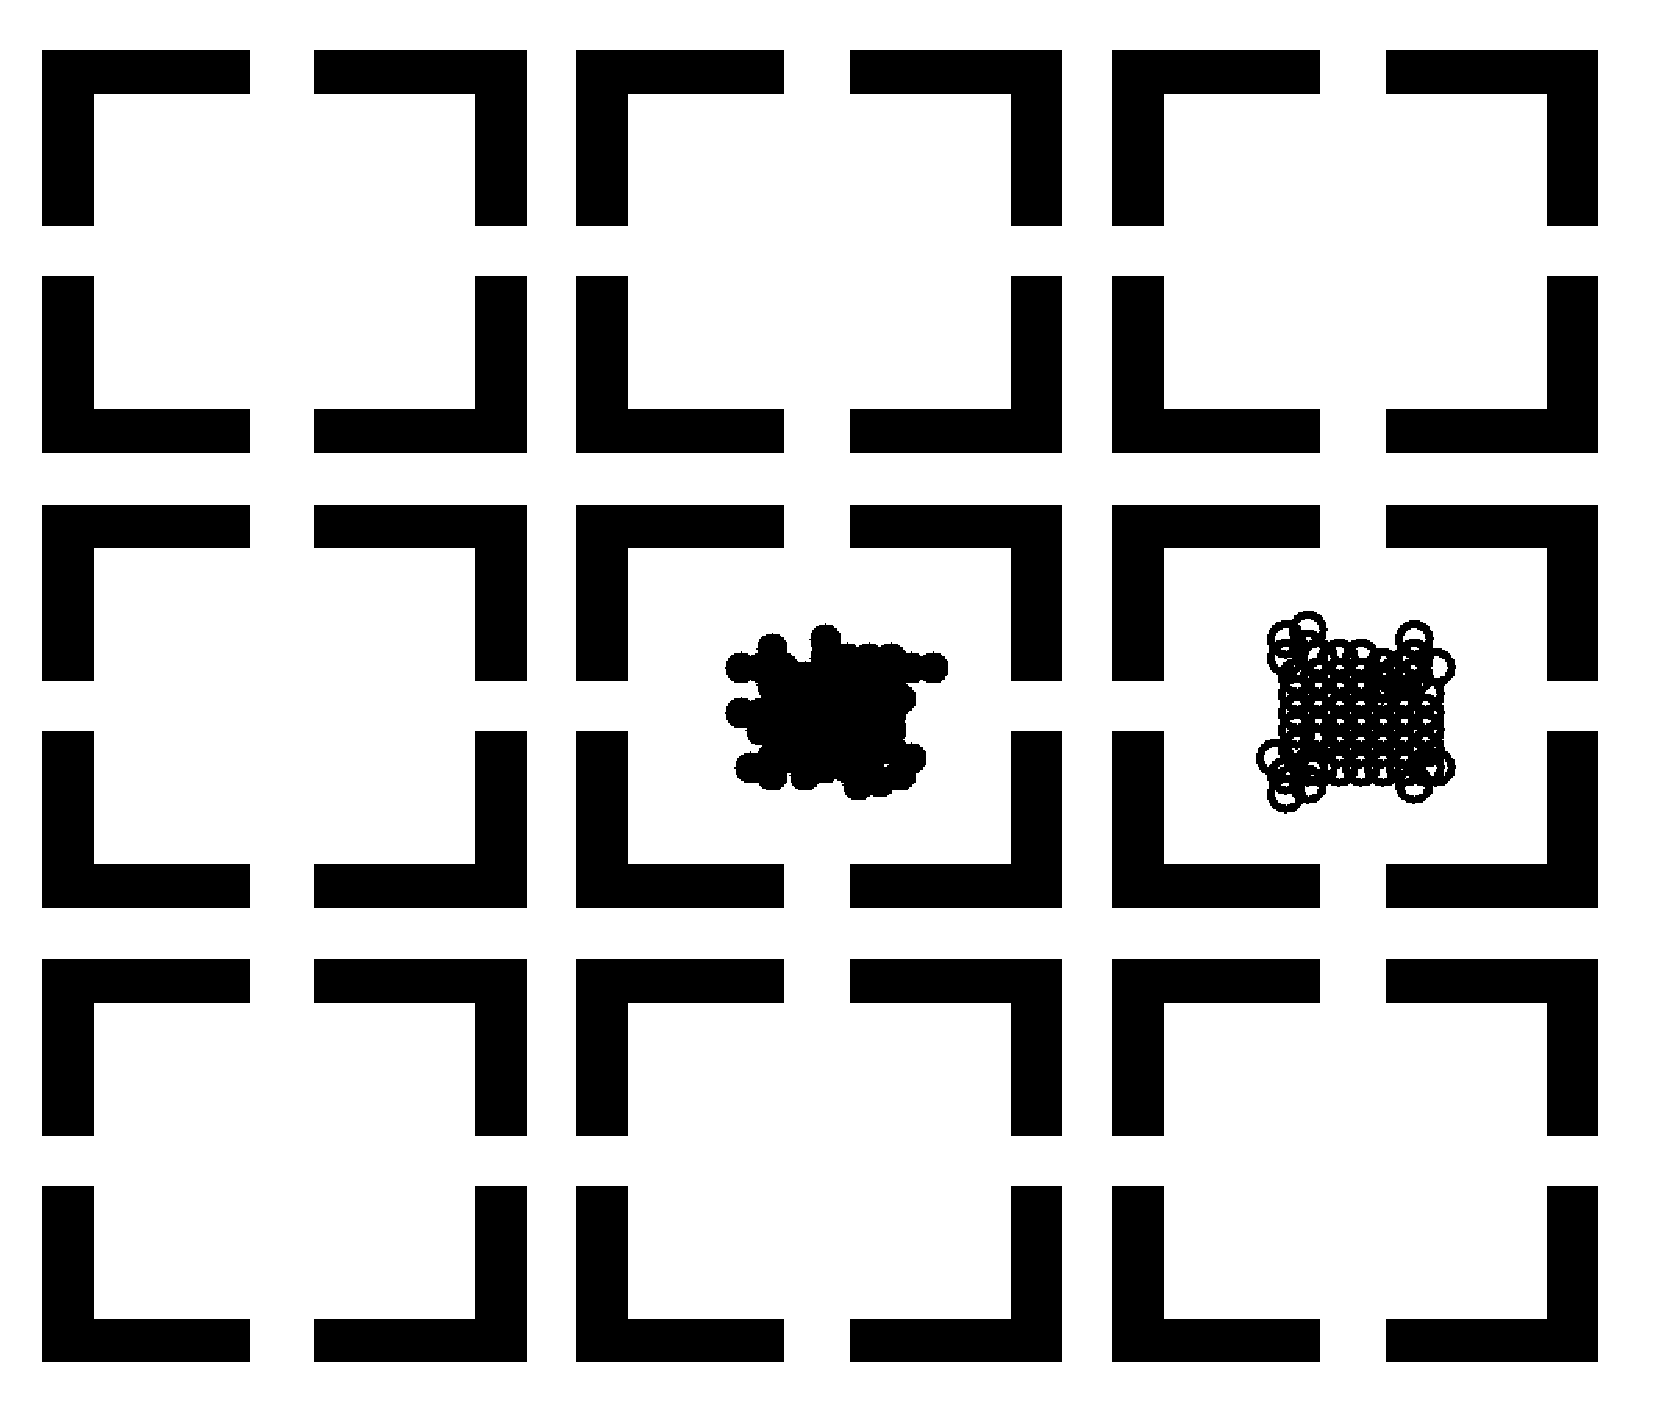
\includegraphics[width=0.3\columnwidth]{img/jos-snapshots/2-4}
    \caption{A run showing the effect of crowding: dark visitors occupy a central room, making other visitors moving left to right by a longer, less crowded path \label{img:museum-generalmap2}}    
\end{center}
\end{figure*}

Both tests show qualitative effectiveness of the proposed laws, and suggest that our simulation approach can be used for additional experiments focussing on tuning system parameters (factor $k$) or alternative strategies (e.g., diffusing crowd information) to optimise paths to destinations.
%
For instance, in the context of the second case, \Cref{img:jos-graph} shows how factor $k$ can influence the time for (sub)groups of (light) people to reach the destination, by which we can see that even small values of $k$ lead to a significant improvement---which slowly decreases as $k$ grows.

\begin{figure}[t]
\begin{center}
   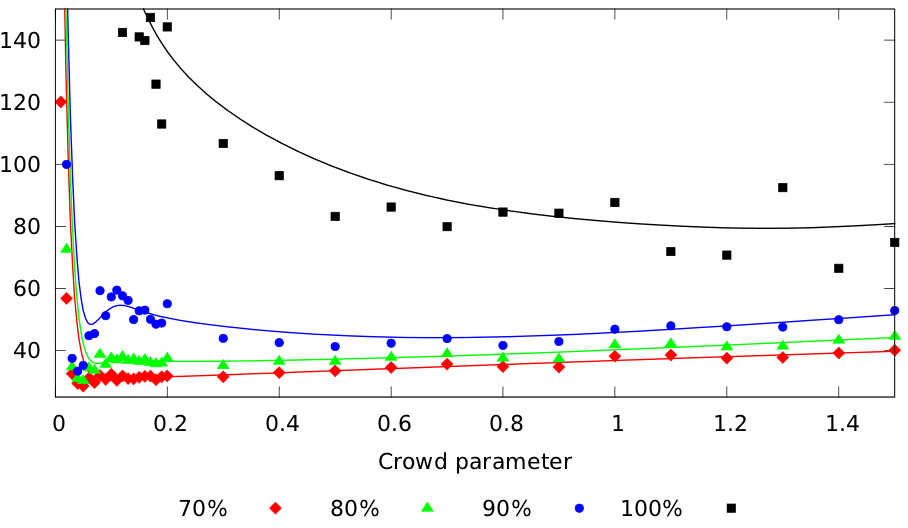
\includegraphics[width=0.99\columnwidth]{img/jos-graph}
   \vspace{-10pt}\caption{Time units of convergence time with different values of crowd parameter and different percentages of people}\label{img:jos-graph}\vspace{-10pt}
\end{center}
\end{figure}


\section{Advanced features}
\subsection{Distributed statistical analysis}
\subsection{Real world maps}

\chapter{Self-organisation patterns}
SAPERE
\section{Crowd evacuation}
\section{Self composition}
\section{Semantic resource discovery}
\section{Anticipative adaptation}
\section{Crowd disasters prediction}
\section{HPC at the urban scale}

\chapter{Aggregate programming languages}
Protelis
\section{Higher order functions in field calculus}
\subsection{Impact on alignment}
\section{Java integration}
\section{Alchemist as a simulation platform}
\section{Alchemist as a core engine for real devices}

\part{Conclusion}
\chapter{Results achieved}

\chapter{Future and ongoing work}
\section{Biochemical meta model for Alchemist}
ciao

%\appendix
%\input{appendix-a.tex}
%\input{appendix-b.tex}
%\input{appendix-c.tex}

%\input{publication.tex}

\part{Bibliography}

%===============================================================================
\small\protect\newpage\addcontentsline{toc}{chapter}{Bibliography}
\bibliography{thesis}
\bibliographystyle{alpha}
%===============================================================================

%\listoffigures
%\listoftables

\end{document}
